% Created 2014-12-17 Wed 16:24
\documentclass[11pt]{template/openetcs_report}
\usepackage{fixltx2e}
\usepackage{graphicx}
\usepackage{longtable}
\usepackage{float}
\usepackage{wrapfig}
\usepackage{rotating}
\usepackage[normalem]{ulem}
\usepackage{amsmath}
\usepackage{textcomp}
\usepackage{marvosym}
\usepackage{wasysym}
\usepackage{amssymb}
\usepackage{hyperref}
\tolerance=1000
\usepackage{todonotes}
\usepackage{pdfpages}
\hypersetup{
  pdfkeywords={},
  pdfsubject={},
  linkbordercolor 	= {1 1 1},
  pdfcreator={Emacs 24.3.1 (Org mode 8.2.4)}}
%===========================
% Graphicpath
%===========================
\graphicspath{{./template/}{.}{./images/}}
%===========================
% Todo note margin
%===========================
\setlength{\marginparwidth}{7em}
%\let\oldmarginpar\marginpar
%\renewcommand\marginpar[1]{\-\oldmarginpar[\raggedleft\footnotesize #1]%
%{\raggedright\footnotesize #1}}
%===========================


\begin{document}
\frontmatter
\project{openETCS}


%assign a report number here
\reportnum{OETCS/WP7/07.3.5}

%define your workpackage here
\wp{Work-Package 7: ``Toolchain''}

%set a title here
\title{OpenETCS Roadmap}

%set a subtitle here
%\subtitle{}

%set the date of the report here


\date{\today}
\title{Traceability Architecture in OpenETCS}
\subtitle{WP7 Proposition}
%define a list of authors and their affiliation here

\creatorname{Cécile Braunstein}
\creatoraffil{University Bremen}
\techassessorname{}
\techassessoraffil{}

\qualityassessorname{}
\qualityassessoraffil{}

\approvalname{}
\approvalaffil{}
\author{Cecile Braunstein}
\affiliation{University Bremen}

\author{Moritz Dorka}
\affiliation{DB}

\author{David Mentré}
\affiliation{Mitsubishi Electric R\&D Centre Europe}

\author{Raphaël Faudou}
\affiliation{Samares Engineering on behalf of ENSEEIHT}


% define the coverart
\coverart[width=350pt]{openETCS_EUPL}

%define the type of report
\reporttype{OpenETCS : Position Paper on traceability}


\begin{abstract}
%define an abstract here
This document presents a proposition to the tool chain traceability
architecture.
\end{abstract}


\maketitle
\tableofcontents

\newpage
%=============================

% The actual document starts below this line
%=============================
%Start here
%=============================
% Document Managment
%=============================
\chapter{Document Information}

\begin{tabular}{|p{4.4cm}|p{8.7cm}|}

\hline
\multicolumn{2}{|c|}{Document information} \\
\hline
Work Package &  WP7  \\
Deliverable ID or doc. ref. & O7.3.5\\
\hline
Document title &Traceability Architecture in OpenETCS \\
Document version & 00.02 \\
Document authors (org.)  & Cécile Braunstein (Uni.Bremen) \\
\hline
\end{tabular}

\begin{tabular}{|p{4.4cm}|p{8.7cm}|}
\hline
\multicolumn{2}{|c|}{Review information} \\
\hline
Last version reviewed &  \\
\hline
Main reviewers &  \\
\hline
\end{tabular}

\begin{tabular}{|p{2.2cm}|p{4cm}|p{4cm}|p{2cm}|}
\hline
\multicolumn{4}{|c|}{Approbation} \\
\hline
  &  Name & Role & Date   \\
\hline  
Written by    &  Cécile Braunstein & WP7-T7.3 Sub-Task  & 06.02.2014 \\
&  & Leader&\\
\hline
Approved by &  &   &  \\
\hline
\end{tabular}

\begin{tabular}{|p{2.2cm}|p{2cm}|p{3cm}|p{5cm}|}
\hline
\multicolumn{4}{|c|}{Document evolution} \\
\hline
Version &  Date & Author(s) & Justification  \\
\hline  
00.00 & 17.12.2014 & C. Braunstein  &  Document creation  \\
\hline  
00.00 & 23.10.2015 & R. Faudou  &  Precisions concerning OpenETCS requirements and models and update of tool chain traceability requirements  \\


\hline  
\end{tabular}
\newpage
%==========================================
\mainmatter
%----------------------
\chapter{Introduction}
\section{Document purpose}
This document presents a proposition concerning support of openETCS project traceability activity by openETCS tool chain. This proposition is a consensus between traceability needs, project policy (open source solutions), time and efforts (focus on existing tools and features) and risks about tool maturity.

\section{Document scope}
This proposition is based on the needs and priorities about traceability, captured from different work packages (mainly WP3 and WP4) during October 2015, either from interviews or from reading of available project documents, especially:
\begin{itemize} 
\item Project Quality Assurance Plan - D1.3 - \cite{qa-plan}.
\item OpenETCS higher level requirements (especially concerning traceability) - D2.6.9 - \cite{D2.6.9}.
\item Definition of OpenETCS Development Process - D2.3a v02 - \cite{D2.3a}
\item OpenETCS Architecture and Design Specification - D3.5.0 - \cite{D3.5.0}  and D3.5.1 - \cite{D3.5.3}
\item Safety plan - D4.2.3 - \cite{D4.2.3}
\end{itemize}

The proposition done in this document is based on existing tools and existing tool capabilities with verified maturity. Document will explain limits of current proposition and will suggest axes to investigate in the future of project (roadmap).
But detailed evaluations of tools and features based on those investigations is not part of this document.

\section{Document organization}
Chapter 2 recalls openETCS project scope, development process, design, VV and Safety processes.

Chapter 3 defines tool chain general requirements concerning traceability driven from \cite{D2.6.9} and from systems engineering experience.

Chapter 4 refines short term development design process and main priorities to deliver demonstrators for ITEA2 project. It provides detailed practical scenarios and expected support on verification and especially traceability during the different phases of development process.

Chapter 5 presents current traceability architecture defined to support practical scenarios identified in chapter 4 for short term development target. This architecture is based on use of existing tools/features.

Chapter 6 summarizes limits of the current traceability architecture and suggests axes to investigate in order to improve traceability support by the OpenETCS tool chain.

\chapter{OpenETCS traceability context}

Requirement traceability concerns relations between requirements existing at different engineering levels and relations between requirements and design or verification engineering artifacts that can exist through different formats (models, documents, code...).  

Before describing the way openETCS tool chain supports creation and maintenace of traceability links, it is important to clearly define the scope of openETCS activity and the artifacts that we want to trace over project life cycle. Next paragraphs recall OpenETCS vision,  development process and current scope of development.

\section{Recall of OpenETCS target vision and development process}
\label{OpenETCS scope}
\cite{D2.3a} mentions that openETCS activity pursues the vision of a full CENELEC compliant development of open-source software for the \emph{European Vital   Computer} (EVC). It is intended to produce a software kernel which can be used in commercial EVCs.

CENELEC 50128:2011 is the relevant engineering standard for software development of safety-critical rail systems. It is completed with CENELEC 50126-1:1999 to address system and subsystem engineering activities required to prepare software development with system requirements. 


\cite{D4.2.3} recalls that \textit{the main products of the openETCS project will be the openETCS specification model used to generate the openETCS on-board software and the openETCS tool chain development, which is used to formalize the ERA Specifications for ETCS, generate the Software Code and perform verification and validation activities} 

OpenETCS software development process reflects this model-based approach while remaining compliant with CENELEC engineering standards. 

\begin{figure} [htbp]
\centering
\includegraphics[width=.9\linewidth]
{./images/OpenETCSDevelopmentProcess.png}
\caption{\label{fig:OpenETCSDevelopmentProcess}OpenETCS software development process}
\end{figure} 

\section{OpenETCS project context-of-interest}
\label{OpenETCS_ITEAProjectScope}
\cite{D3.5.3} recalls last refinement of project scope concerning functional coverage: "OpenETCS project has decided not to consider all ETCS subsystems and to tailor scope to cover the functionality required for the openETCS demonstration as an objective of the ITEA2 project. The goal is to develop a formal model and to demonstrate the functionality during a proof of concept on the ETCS Level 2 Utrecht Amsterdam track with real scenarios".

Figure \ref{fig:openETCSSystemOfInterest} details ETCS system scope to consider in order to cover expected demonstration of EVC software for ITEA project. Scope is highlighted in ERA TSI chapter 2 and provides basis for System detailed analysis and functional breakdown.

\begin{figure}[htbp]
\centering
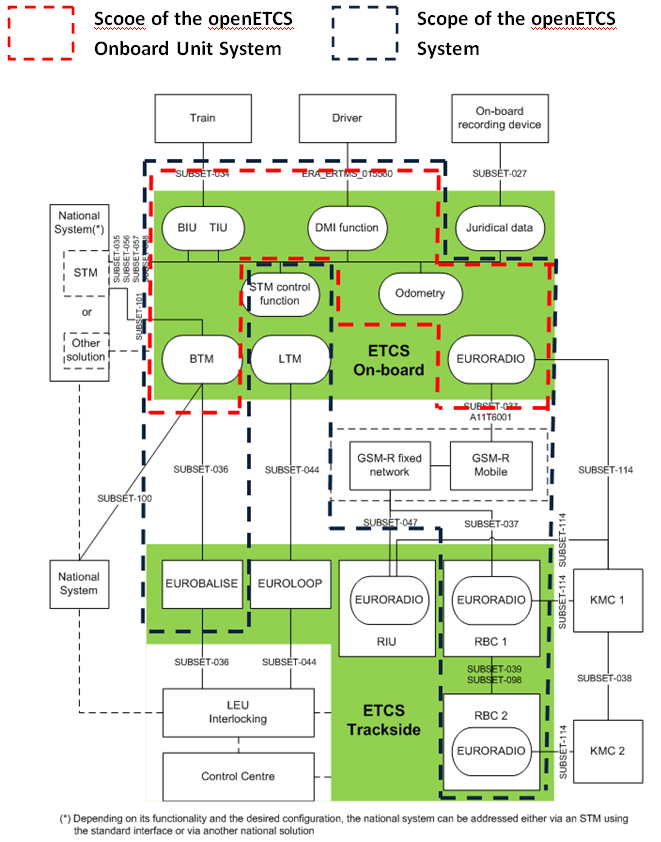
\includegraphics[width=.9\linewidth]{./images/ArchitectureSRS.PNG}
\caption{\label{fig:openETCSSystemOfInterest}OpenETCS system of interest (dotted black line) to cover demonstration objective of ITEA2 project and according to ERA TSI Chapter 2}
\end{figure}

\section{OpenETCS design process (WP3) and design artifacts}
\label{InterestOfReferenceEngineeringArtefacts}
After recalling the development process and precising openETCS project scope we must now look at the design process to see which artifacts are produced to meet openETCS requirements. This process is under WP3 responsibility.

\label{DesignProcessStrategy}

At system level (ETCS), we have to produce two main specifications: Elaborated System Requirements Specification and System Architecture Design Specification.

As recalled by \cite{D3.5.3}, first idea was to formalize SRS subset 026 on the scope defined previously and then continue system decomposition from this formalization. But from experience of openETCS partners, this approach is not sufficient in order to fully understand the main issues related to the SRS.
So, instead of building yet another copy-paste direct formalisation of the ETCS SRS, WP3 suggested another approach using a SRS functional analysis centred on Onboard unit and focused on the reference track (ETCS L2 Utrecht- Amsterdam).

This approach leads to the following architecture and design artifacts described in \cite{D3.5.0} :
\begin{itemize} 
\item User story models that refine textual user stories about use of OBU in operational context: done with SysML language and Papyrus tool. It provides another entry for project stakeholder requirements and prepares validation.
\item System Architecture model, defined with SysML language and Scade system Designer tool, with currently two decomposition levels: 
		\begin{itemize} \item System breakdown structure, centred on ETCS OBU and defining required interactions to other ETCS subsystems (external interfaces)
		\item Functional breakdown from OBU, centred on ETCS Kernel and defining functional interactions between those internal functions (internal interfaces, mainly data flow)
		\end{itemize} 

\item OpenETCS application software executable model, a model defined with SCADE tool. This model integrates several behavioral SCADE models that realize functional block interfaces identified in SysML Architecture model
\item Environment model, designed with SCADE tool and SCADE display for simulation HMI, that supports validation of OpenETCS application software executable model
\item OBU SW Architecture and Design Document (ADD) providing a functional description of software architecture and design
\item A RFC (Request For Comment) process that provides a cross-reference to the SRS, listing
all requirements and design conflicts that have been identified during work. 

\end{itemize}

Figure \ref{fig:OpenETCSArchitectureAndDesignModel} illustrates the architecture breakdown performed in openETCS architecture model starting from ETCS system down to ETCS kernel software component.


\begin{figure}[htbp]
\centering
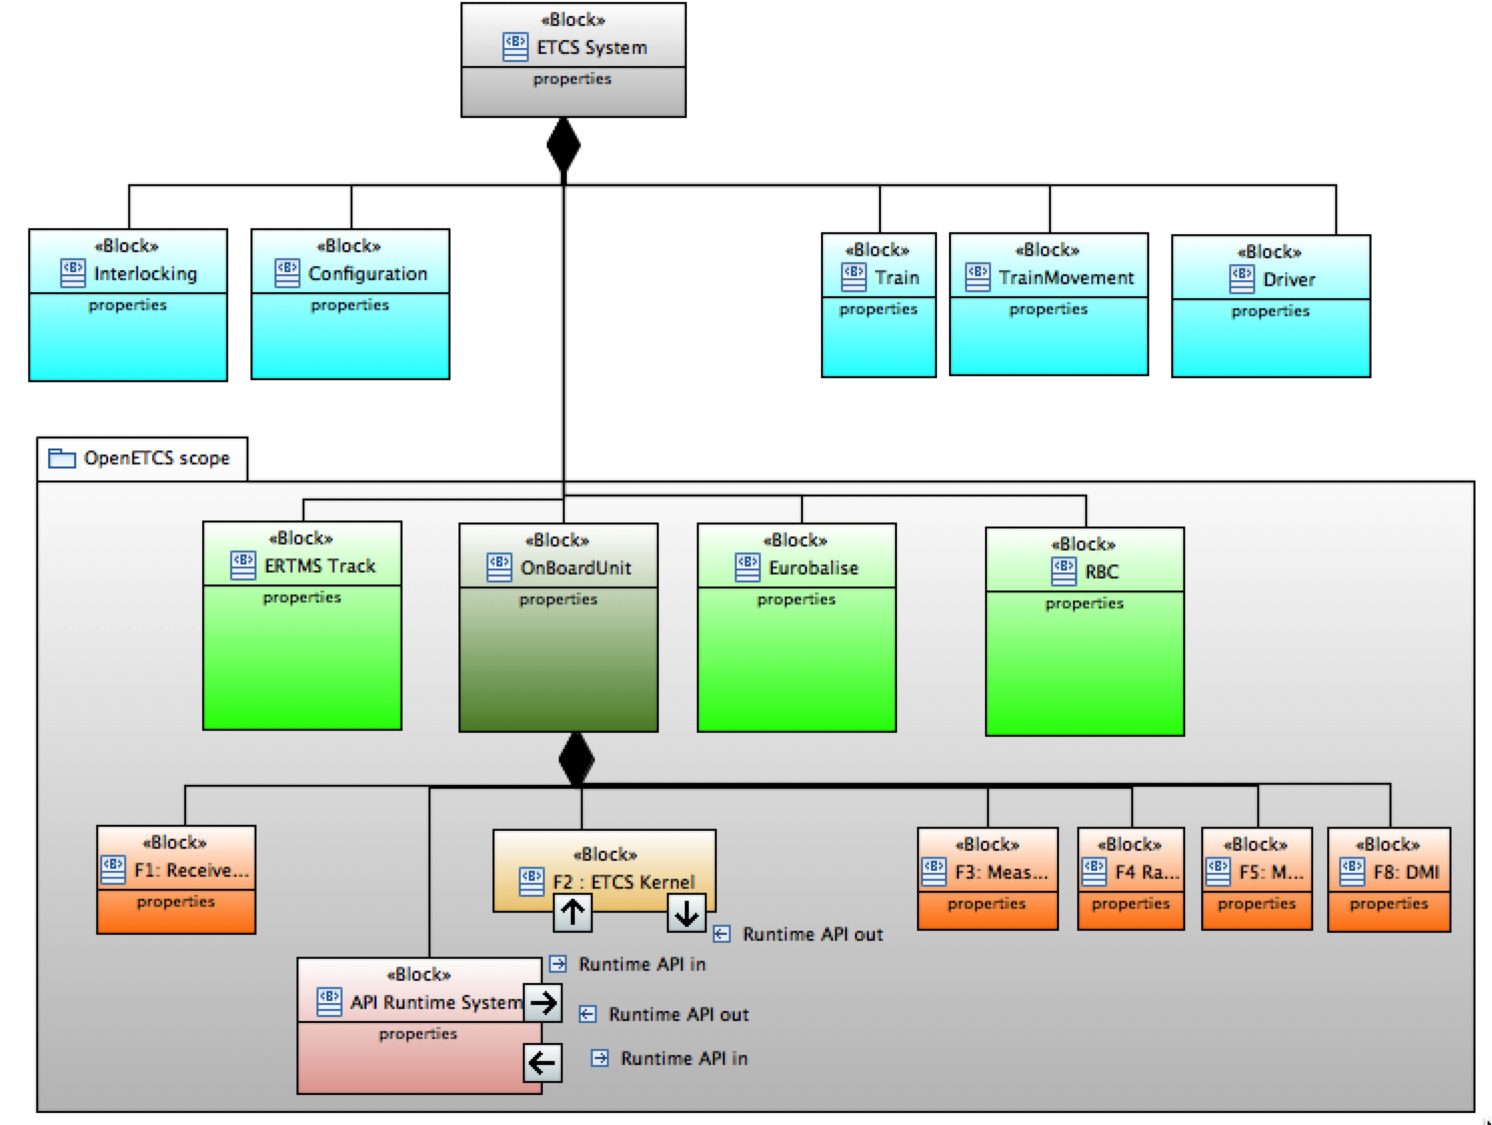
\includegraphics[width=.9\linewidth]
{./images/OpenETCSArchitectureAndDesignModel.png}
\caption{\label{fig:OpenETCSArchitectureAndDesignModel}OpenETCS architecture with SysML: from system to software components}
\end{figure}

Figure \ref{fig:WP3DesignProcess} summarises design process defined by WP3 and shows relations between different design documents and with reference input artifacts: SRS subset26, Utrech-Amsterdam reference track scenarios and openETCS API for platform interoperability. Black arrows mean "input for" while red arrows are traceability relations to reference artifacts.

\begin{figure}[htbp]
\centering
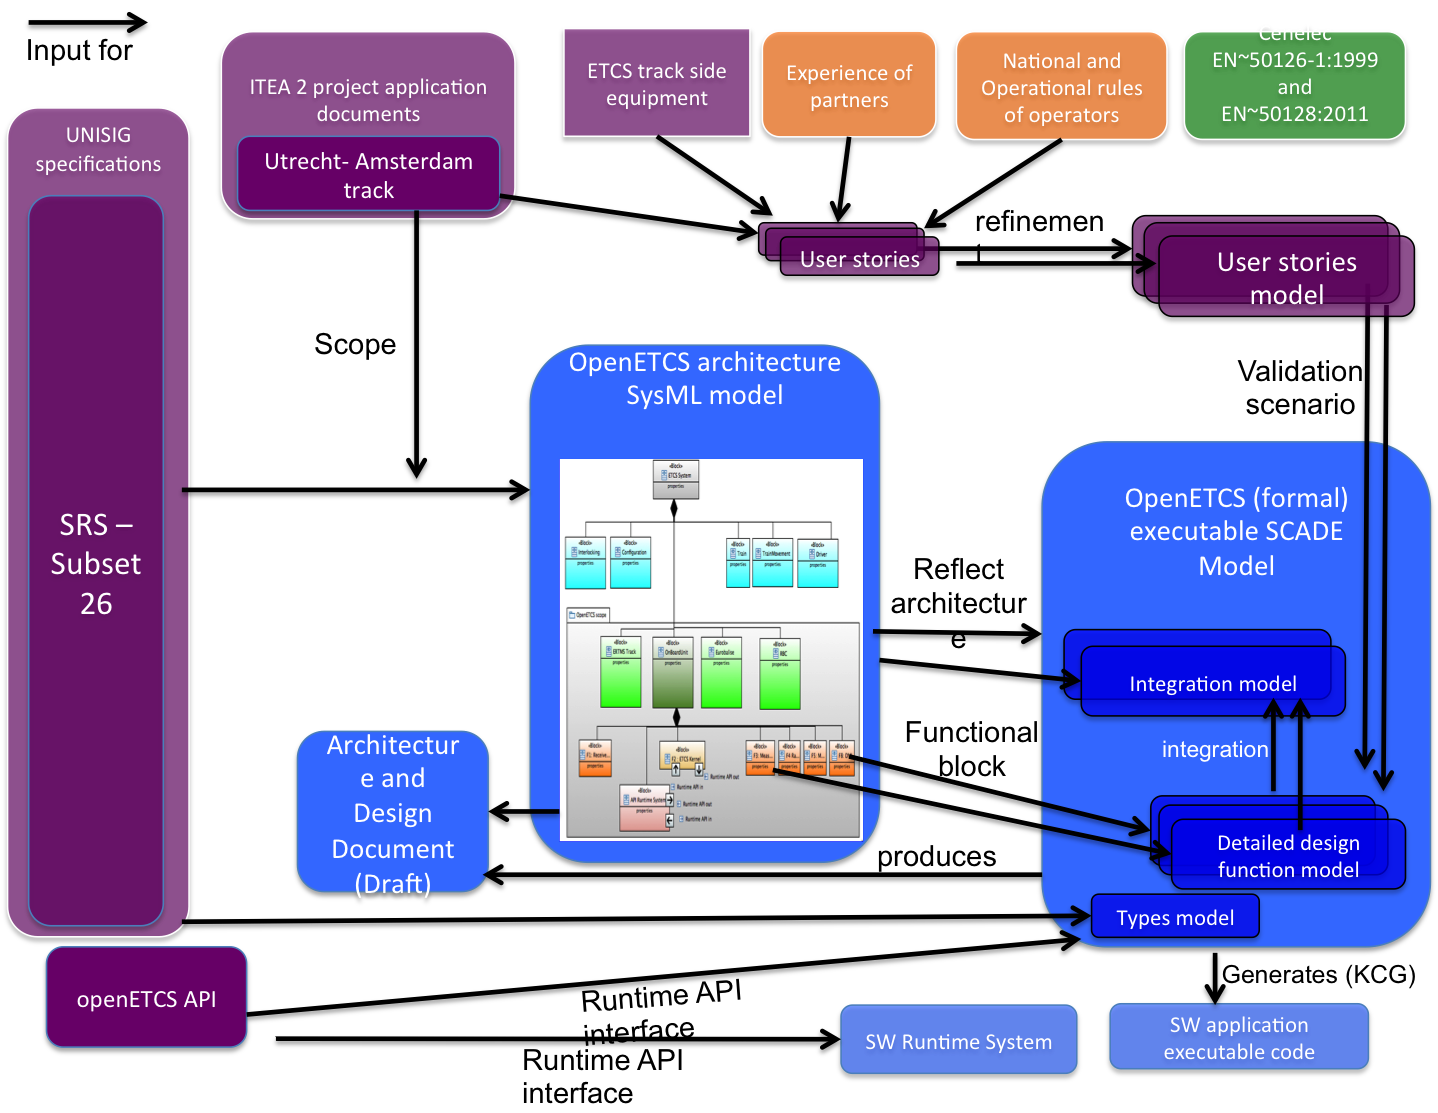
\includegraphics[width=1.0\linewidth]
{./images/WP3DesignProcess.png}
\caption{\label{fig:WP3DesignProcess}Relations between main WP3 Design Documents and reference input artifacts (SRS, Utrecht-Amsterdam reference track and OpenETCS API)}
\end{figure}

\section{OpenETCS VV and safety process (WP4)}


\cite{D4.2.3} recalls that the openETCS software development has to interact with a respective generic safety management process and take the overall safety requirements for a train control system into account. 

During validation of product, OpenETCS project has to provide a safety case. 
The openETCS safety case shall present a transparent and easy to follow argumentation chain
connecting the system definition with all basic safety assumptions and all evidence. To do this it
has to show the relations between design and V\& V artifact created during the iterative openETCS
development process. Thereby, it has to be shown to which degree and under which assumptions
the resulting documentation covers process, quality and safety requirements based on EN 50126,
EN 50128 and EN 50129.

Figure \ref{fig:SafetyProcess} shows the interactions between design, verification and validation and the general quality and safety management.

\label{safetyProcessApplication} 
Concerning application of safety process in the scope of openETCS ITEA project, it is not possible to apply it on full scope of the project with all requirements expressed in CENELEC engineering standards .
So a proof of concept has been defined in order to apply it with a model based approach. PoC is based on Management of Radio Communication (MoRC).
Results are available here: https://github.com/openETCS/validation/tree/master/VnVUserStories/VnVUserStoryAll4Tec-AEbt but safety requirements have not been integrated into the project requirements database (.ReqIF files).

But this PoC has demonstrated feasibility and usefulness but has not been extended to the full scope of project. 




\begin{figure}[htbp]
\centering
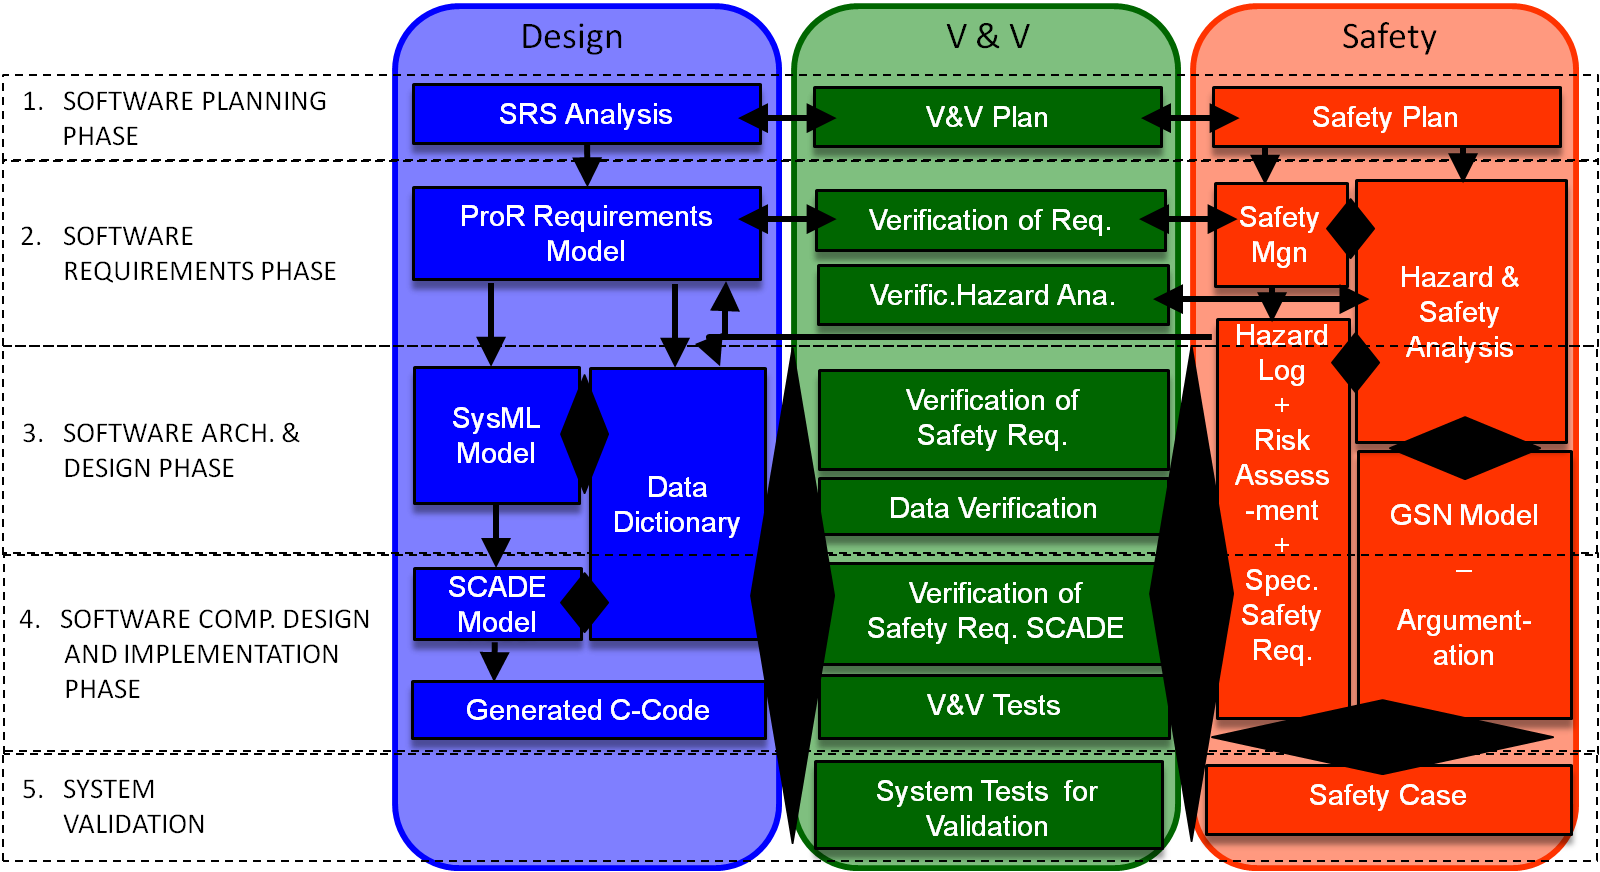
\includegraphics[width=1\linewidth]{./images/openETCS-Software-Safety-Development.png}
\caption{OpenETCS development relations between design, verification and validation and safety activities}
\label{fig:SafetyProcess}
\end{figure}

\chapter{OpenETCS tool chain general requirements about traceability}
\label{sec-2} 

This chapter starts by recalling openETCS tool chain high level requirements concerning traceability. They have high priority as reference inputs for the project.

But we will see that those requirements are hard to apply "as-is" because they address generic artifacts with undefined scope and poorly defined semantics. So we discuss them and then complete them with more practical tool chain capabilities derived from systems engineering experience about traceability and first expectations already captured from introduction. 


\section{OpenETCS high level requirements about traceability support by tool chain}
\cite{D2.6.9} defines a set of high level requirements for the project including some concerning tool chain. Among them we find R-WP2/D2.6-02-079 that addresses traceability support through a set of sub requirements. We recall them below.

R-WP2/D2.6-02-079 The tool chain shall allow traceability between:
\begin{itemize}
\item R-WP2/D2.6-02-079.01 the documentation/requirements and the models,
\item R-WP2/D2.6-02-079.02 the documentation/requirements and the tests,
\item R-WP2/D2.6-02-079.03 the models and the tests,
\item R-WP2/D2.6-02-079.04 each required level of implementation and the lower level (e.g. higher
level model vs lower level model, lower level model vs source code. . . ),
\item R-WP2/D2.6-02-079.05 the documentation/requirements and the models,
\item R-WP2/D2.6-02-079.06 the documentation/requirements and the safety properties/requirements,
\item R-WP2/D2.6-02-079.07 the models and the safety properties/requirements,
\item R-WP2/D2.6-02-079.08 the tests and the safety properties/requirements.
\end{itemize}

\subsection{Which model?}
A model, even if we restrict it to the context of systems engineering,  may have a lot of purposes including formalization of requirements, architecture definition, property verification or simply illustration of concepts for communication. 

Figure \ref{fig:TypologyOfSystemsEngineeringModels} suggests a possible typology of systems engineering models that illustrates the wide range of model purposes.

\begin{figure}[htbp]
\centering
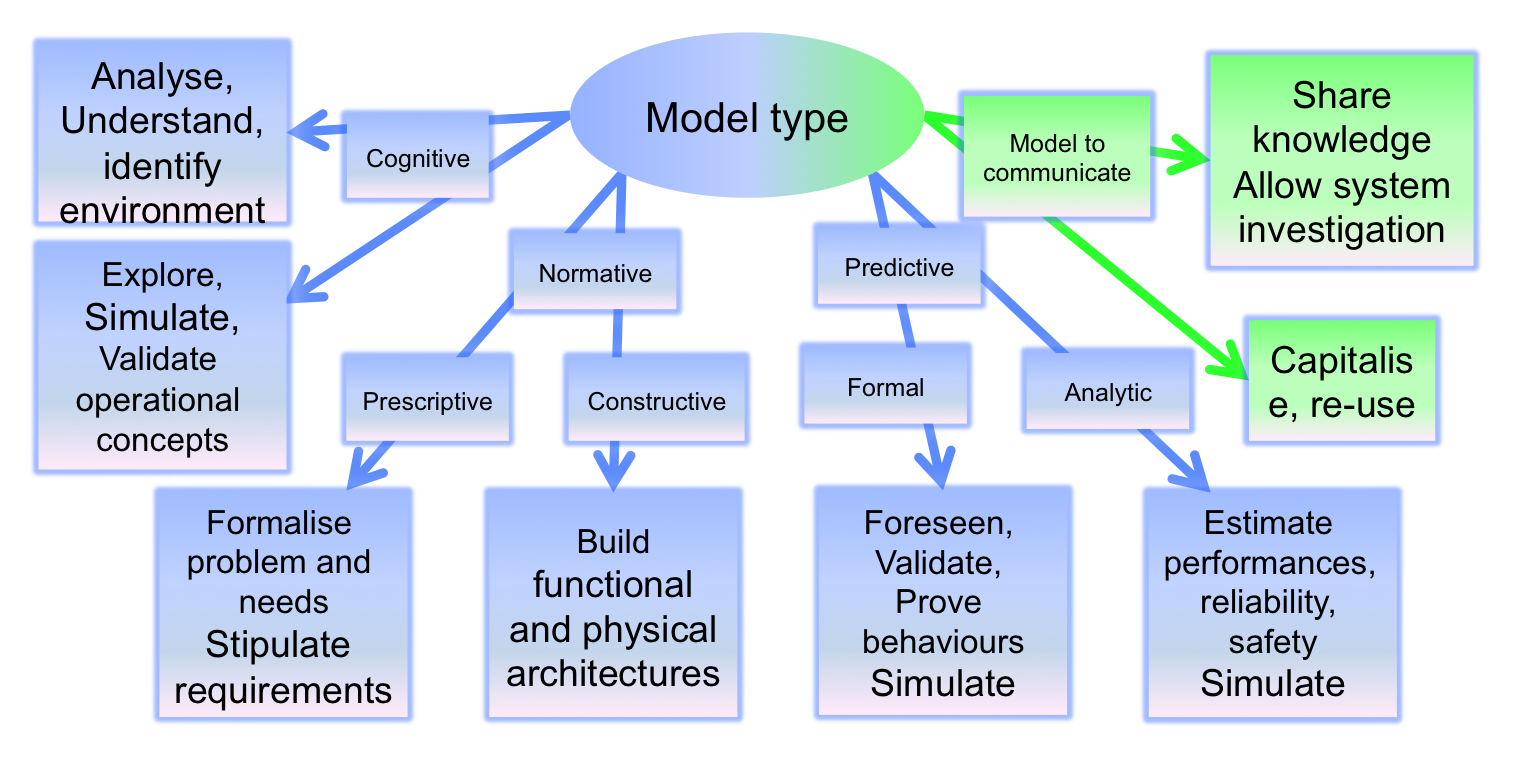
\includegraphics[width=.9\linewidth]
{./images/TypologyOfSystemsEngineeringModels.png}
\caption{\label{fig:TypologyOfSystemsEngineeringModels}Possible typology of systems engineering models}
\end{figure}

According to its purpose and intended use in the development process, a model can be considered as a reference engineering artifact maintained in configuration or as an intermediate means that helped building some engineering artifact but that can be thrown away after some time.

As creation (and maintenance over time) of traceability links is time and efforts consuming and we suggest restricting it to models that are or contain key engineering artifacts (configuration items).

With that precision, requirement D2.6-02-079.01 would then become: "the tool chain shall allow traceability between documentation/requirements and the models that are or contain configuration items"

\subsection{What does "tracing model" mean?}
Tracing a model is generally not at the right scope. More precisely we want to trace artifacts contained in a model (like block properties, state transitions, data flow...). So we need to be able to identify those artifacts in the model and to name them unambiguously, with clear context (position/hierarchy in the model) and unique name.


\section{Tool chain capabilities to support requirement management}
\label{ReqMgtCapabilities} 
Requirement traceability cannot be fully supported by tool chain if there is no ability to manage requirements (create, edit, visualize, classify...) as expressed in previous chapters through main scenarios.

Requirement management is an activity that consists in supporting different tasks concerning requirements during the project, whatever the engineering level. In OpenETCS project we need at least the following commands available in the tool chain (and potentially restricted according to access rights if defined):
\begin{itemize}

\item Visualization of one or several requirements, their links if any and their attributes. 
\begin{itemize} \item \textbf{OpenETCS example}: visualize one Subset026 SRS or API requirement, its statement and its hierarchy (father requirement if any and children requirements if any).
	\item \textbf{OpenETCS example}: visualize one openETCS software requirement, its statement and upstream traces up to Subset 026.\end{itemize}

\item Query (filter, ordering) on a set of requirements with filter based on requirement attribute values or on links between requirements
\begin{itemize} \item \textbf{OpenETCS example}: list only subset026 SRS chapter 7 requirements that are not yet traced (no traceability link)	\item \textbf{OpenETCS example}: list OpenETCS SW requirements that are not yet traced (no traceability link).
\end{itemize}

\item Creation and storage of requirement and of different attributes based on a given requirement template/type, in a given requirement hierarchy and with unique identifier allocation based on a flexible (customizable) strategy
\begin{itemize} \item \textbf{OpenETCS example}: creation of a new openETCS requirement decomposed from a susbet026 SRS requirement, from risks and hazards analysis (safety requirement) or from software design. Newly created requirement shall have unique identifier automatically allocated to be consistent with its hierarchy (father requirement id) and with an attribute "maturity" set to "to be confirmed" and creation date set to the current date.
\end{itemize}

\item classification of one or several requirements into engineering levels (scopes) that can be defined by end users.
\begin{itemize} \item \textbf{OpenETCS example}: allocation of a newly created requirement to the OpenETCS system level, Onboard Unit SW level, OB SW component level or OBU SW component interface level .\end{itemize}

\item Edition of one or several requirements and their attributes
\begin{itemize} \item \textbf{OpenETCS example}: confirmation of a newly created requirement with attribute "maturity" set to "confirmed".\end{itemize}

\item Addition of a version on one requirement or on a set of requirements
\begin{itemize} \item \textbf{OpenETCS example}: selection of a set of reviewed openETCS requirements of a given scope (level) and addition of a version for all those requirements.\end{itemize}

\item Ability to compare two versions of a set of requirements and list all requirements that have been added or modified.
\begin{itemize} \item \textbf{OpenETCS example}: comparison of two versions of Subset026 SRS requirements (system input activities) or two versions of OBU SW requirements and visualization of all requirement links to check.\end{itemize}

\item Import of requirements coming from external sources (ReqIF, Word, Excel...)
\begin{itemize} \item \textbf{openETCS example}: import of Subset026 Word document (System specification activities) or ReqIF format (OBU SW requirements). Import of openETCS API definition.\end{itemize}

\item Export of a set of requirements to another format: at least ReqIF standard interchange format but also office format (.csv, excel or word...) \begin{itemize} \item \textbf{OpenETCS example}: export of all openETCS created requirements and links into .csv file \end{itemize}

\end{itemize}

In addition, requirement management tooling shall enable share and access of requirements within a team, through a shared repository (shared directory on a network drive or CVS repository like SVN, Git, ClearCase or any other one): either directly (all team members access same shared repository) or with local work and synchronizations between team members through a shared repository.

\section{Tool chain capabilities to support requirement traceability}
\label{TraceabilityCapabilities} 
Requirement traceability activity consists in ensuring that all product engineering artifacts (including verification means) can be traced to an originating stakeholder requirement either directly (direct link) or through other requirements derived from stakeholder requirements. It means creating links but also manage their status (created, confirmed...) and potentially their deletion.

In order to support this activity in openETCS project we need at least the following commands available in the tool chain:

\begin{itemize}

\item Creation of a link between a requirement and an engineering artifact, based on a given link template/type (refine, derive, implement, verify...). 
\begin{itemize} \item \textbf{OpenETCS example}: create a "Satisfy" link between one openETCS SW functional requirement and one OnBoard Unit function, with  "status" link attribute set to "defined" and "rationale" attribute set with appropriate justification.\end{itemize}

\item edition of link status. 
\begin{itemize} \item \textbf{OpenETCS example}: after review, confirm some traceability links  by setting "status" attribute to "validated" value.
	\item \textbf{other OpenETCS example}: after change in some openETCS SW requirements, for all traceability links of modified requirements, set status to "to check" value.\end{itemize}

\item deletion of requirement traceability link. 
\begin{itemize} \item \textbf{OpenETCS example}: after review, decide that some traceability links are not accurate and delete them.\end{itemize}

\item export of requirement traceability
\begin{itemize} \item \textbf{OpenETCS example}: after progress meeting, export current requirement traceability to .csv file so that it can be analyzed by project manager and/or quality team\end{itemize}

\end{itemize}


\chapter{Short term development priorities and associated practical scenarios concerning traceability}

OpenETCS activity targets long term objectives (recalled in introduction) but has also to fulfill short term target with demonstrators for ITEA2 project within limited remaining efforts and time. 
This chapter explains the priorities put on development (design and verification activities) to reach this short term target and provides practical scenarios with focus on traceability.

\section{Main design priorities and current requirement organization}
From WP3 point of view, most important development chain concerns ETCS OBU formal model and its links to the Subset026 SRS requirements and all other requirements created during system analysis, either by decomposition, refinement or derivation. 
ETCS OBU model is detailed down to software detailed design level, and as it is a formal model, it becomes possible to generate code from that model. So, if it is possible to demonstrate that this model satisfies some SRS Subset 26 requirements, then it will be possible to establish that software code generated from that model also satisfies those requirements.

Full process recommended by CENLEC engineering standards implies deriving all stakeholder reference requirements (including SRS subset 26 , openETCS API and user stories) into OpenETCS requirements layered in system, subsystem and software levels.
See figure \ref{fig:idealRequirementOrganization} for ideal requirement management organization.

\begin{figure}[htbp]
\centering
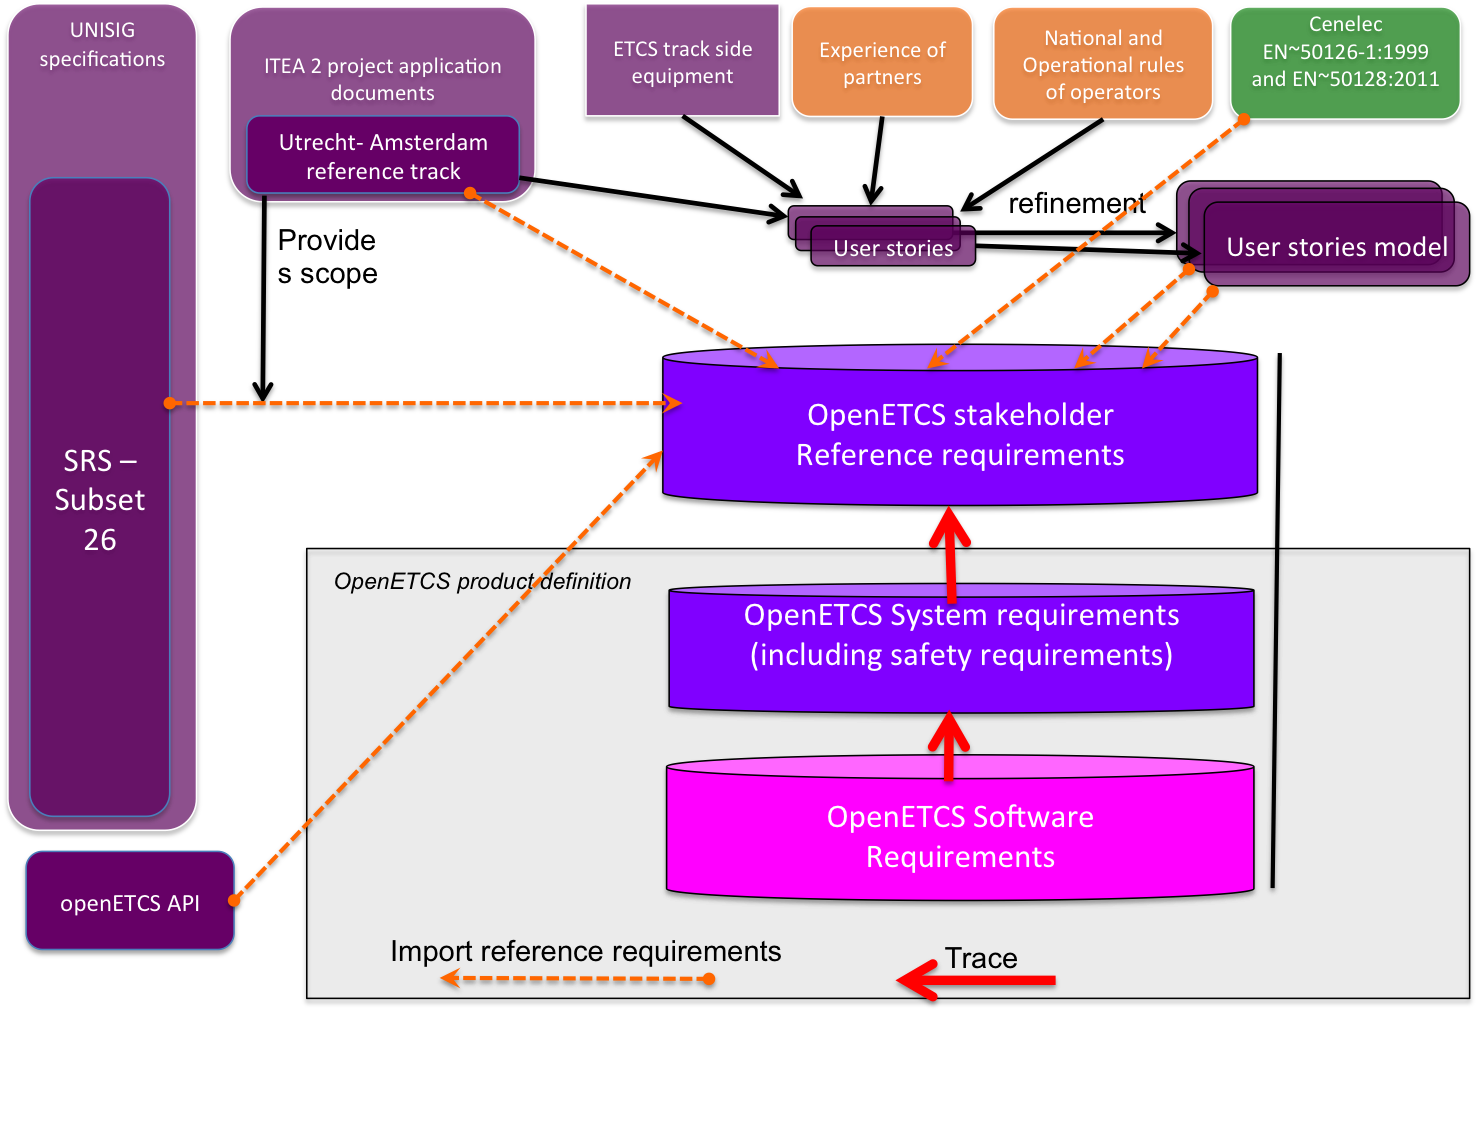
\includegraphics[width=1\linewidth]{./images/idealRequirementOrganization.png}
\caption{OpenETCS ideal requirement management organization}
\label{fig:idealRequirementOrganization}
\end{figure}

But most openETCS requirements starting from ETCS system down to software level are already present in SRS subset 26 through the different chapters. So requirement analysis and derivation process mainly leads to propagating existing requirements from SRS subset 26 document to OpenETCS requirements and the value of such transformations is low compared to the efforts for propagation and allocation to levels. So idea is to use SRS subset 26 as openETCS requirements and use the chapters structure to differentiate between levels. They are translated into .reqIF format so that requirements can be managed by requirement management tools. Other reference requirements are imported in the openETCS reference configuration (baseline) as documents.

Figure \ref{fig:CurrentRequirementOrganization} illustrates current organization for requirement management.

\begin{figure}[htbp]
\centering
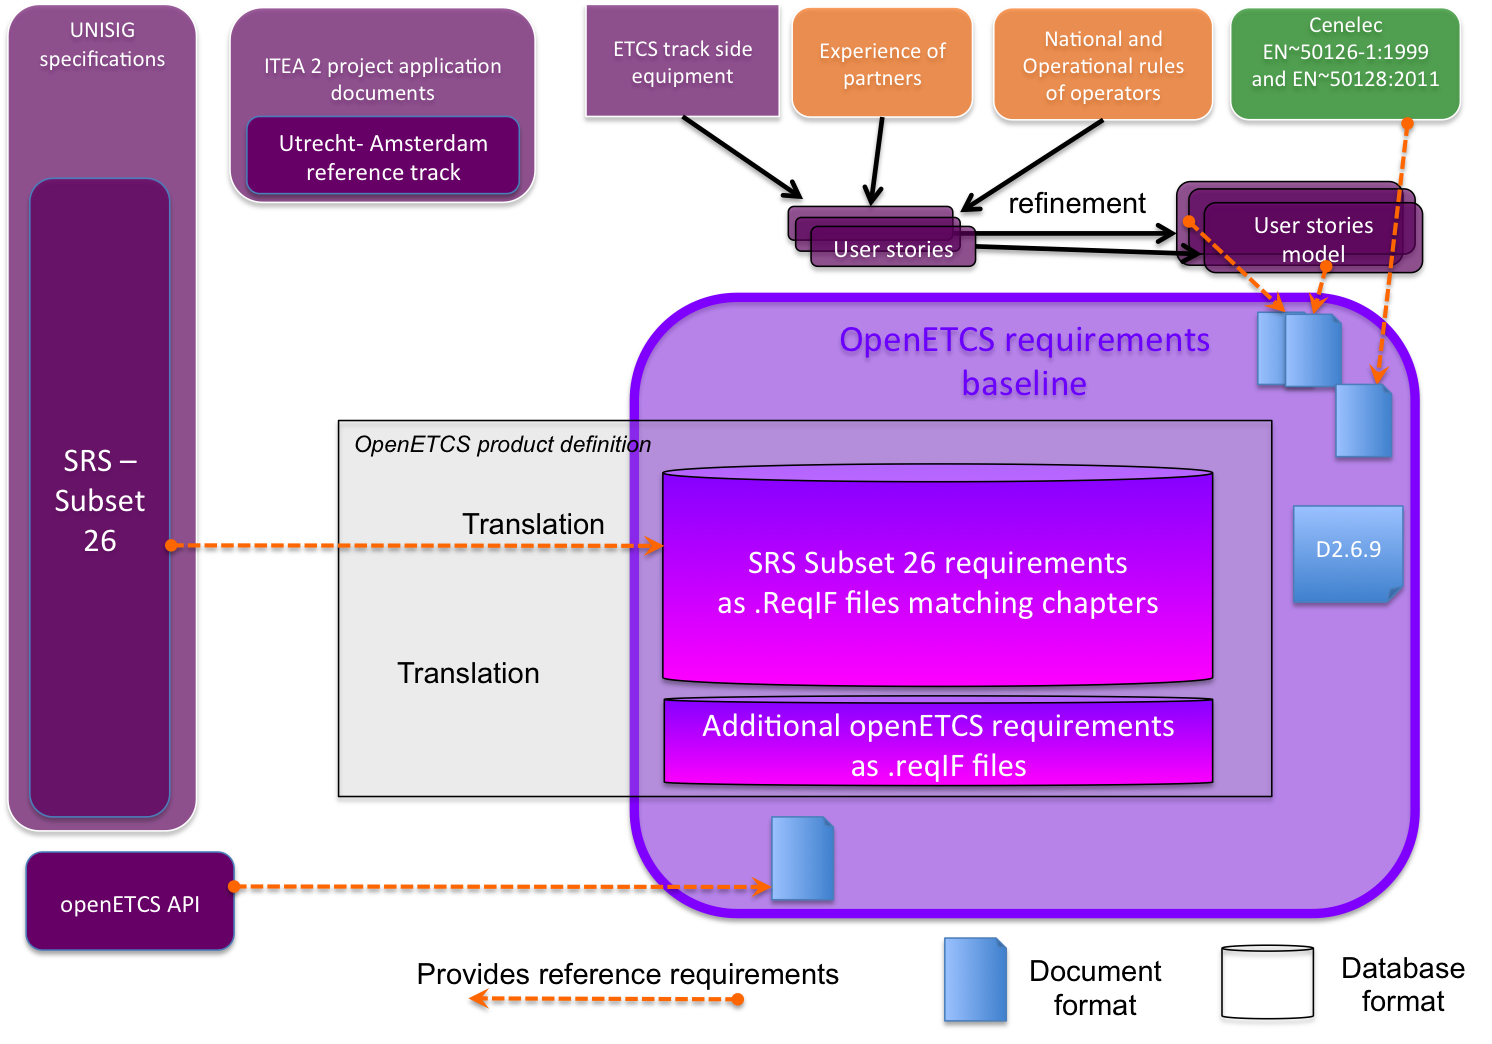
\includegraphics[width=1\linewidth]{./images/CurrentRequirementOrganization.png}
\caption{OpenETCS current requirement management organization}
\label{fig:CurrentRequirementOrganization}
\end{figure}


SysML model, used to capture and describe architecture from System level down to software internals, is considered as an intermediate means in the sense that it helps producing the OBU scade formal model but might be not maintained once OBU model is finalized and can be traced directly to the SRS Subset 26. 

But currently, SysML model plays a role in this definition and so we need to create traceability links with it so that we can verify that architecture conforms to the SRS subset 26.

Figure \ref{fig:openETCSTraceabilityMainPriority} illustrates all required traceability links needed to achieve current design verification and highlights those conisdered with highest priority (arrows with largest size) for short term.

\begin{figure}[htbp]
\centering
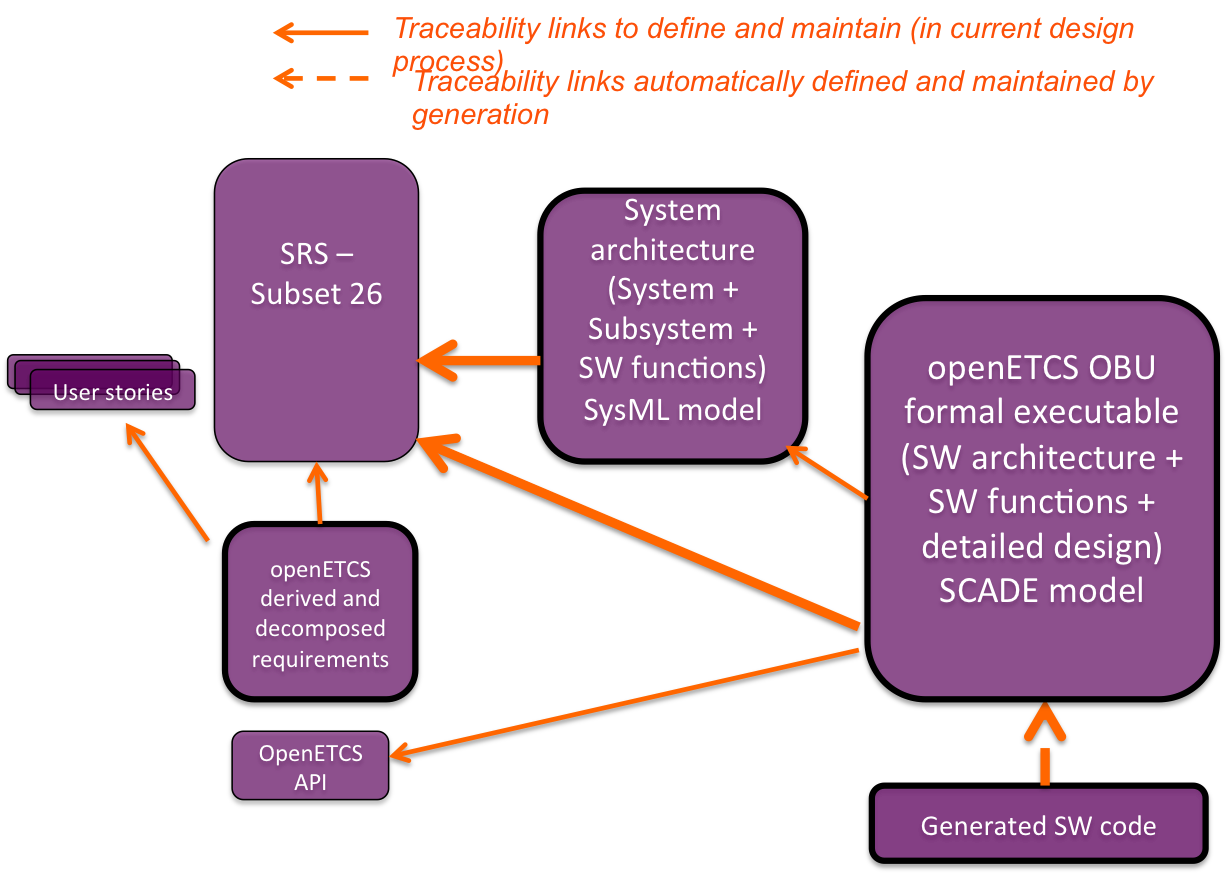
\includegraphics[width=.9\linewidth]
{./images/openETCSTraceabilityMainPriority.png}
\caption{\label{fig:openETCSTraceabilityMainPriority}OpenETCS traceability chains for current design with highlight on main priorities}
\end{figure}

Next paragraphs explain traceability during the 5 phases of the software development process with specific focus on links between openETCS OBU model and SRS Subset 26.


\section{OpenETCS traceability main scenarios}
Traceability main scenarios are grouped by phase according to the openETCS software development process introduced in previous chapter. 

We recall illustration of software development process below to ease reading of next paragraphs.

\begin{figure} [htbp]
\centering
\includegraphics[width=.9\linewidth]
{./images/OpenETCSDevelopmentProcess.png}
\caption{\label{fig:OpenETCSDevelopmentProcess}OpenETCS software development process}
\end{figure} 

\subsection{P1 Software specification Phase}

\cite{D4.2.3} recalls P1 scope and current support for verification.
\textit{The phase P1 Software Requirement Phase covers the development activities required by the EN 50128 during its lifecycle phase Software Requirements Phase (7.2). The SUBSET 26 and further System Specifications are the Input of this work. The resulting ReqIF Requirement files shall represent the Software Requirement Specification. Software Overall Test Specification will be derived with respect to these requirements, but a method is not defined at this point.}

\textbf{Currently .ReqIF Requirement files are translated from SUBSET 26 and there is no derivation or special tag to identify SW requirements. So software overall test specification shall first include this derivation of software requirements in order to conduct test overall SW test specification.}


Note: SysML architecture model provides a good input for such derivation to SW requirements by identifying system, subsystem and SW engineering levels through SysML Block Definition Diagrams and Internal Blocks Diagrams. But currently this model does not lead to the creation of software requirements in the database. 

Figure \ref{fig:P1RequirementDerivationWithSysMLModel} illustrates what could be done.

\begin{figure}[htbp]
\centering
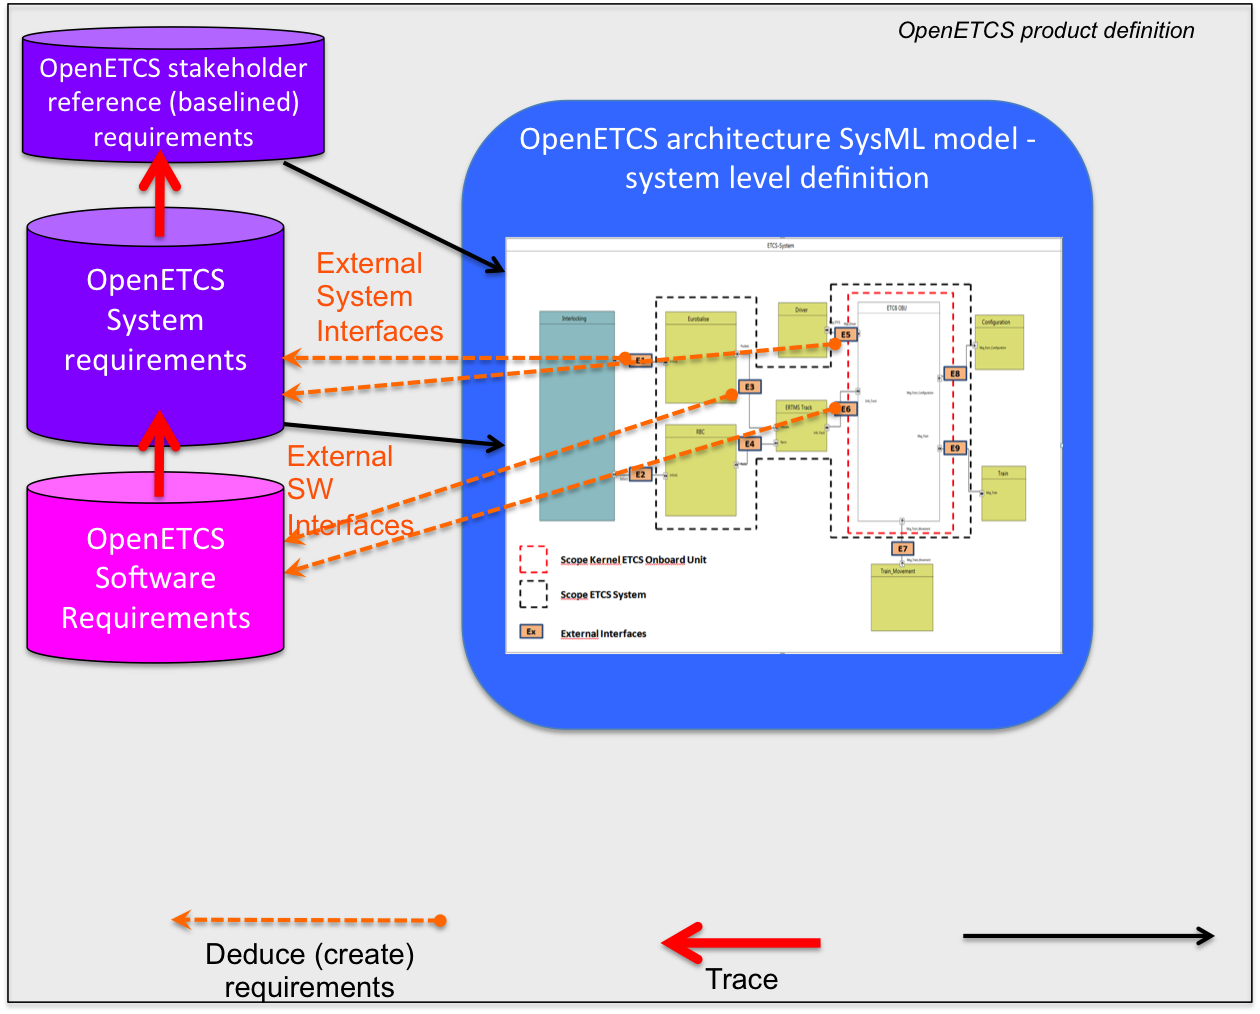
\includegraphics[width=1.0\linewidth]
{./images/P1RequirementDerivationWithSysMLModel.png}
\caption{\label{fig:P1RequirementDerivationWithSysMLModel}Requirement derivation process through SysML architecture model}
\end{figure}

We do not detail this activity and associated traceability because it is not current priority (current priority concerns software verification). However, this derivation process remain important in order to ensure good relevance of software requirements with regards to SUBSET 26 and other system specifications.

Note: concerning Hazard and Risks analysis activity, it has been performed only on a subset of project scope and through a Proof of concept (see \ref{safetyProcessApplication}) that has demonstrated principles and practical feasibility with methods and tools. But this PoC has not yet been extended to the whole scope of project. For short term development, systematic identification of safety requirements and derivation into software requirements are not the main priority now that principles have been demonstrated with success.

Once SW requirements are clearly identified (either created by derivation or tagged in .reqIF files or in other existing documents), it becomes possible to define associated verification means, among test specification, inspection, analysis or certification and associate verification specifications. Those verification specifications shall mention the openETCS concerned SW requirements so that we can check relevance and accuracy. 

In terms of traceability it means that we shall be able to show bi directional traceability between openETCS SW requirements and associated verification specifications. Usual way is to deliver a matrix for that.
Then, reviews can be done with matrix as input to ensure that verification specifications really verify mentioned requirements and that requirements are fully verified by associated verification specifications.
 

\subsection{P2 - Software Architecture Modeling Phase}
The phase P2 covers activities from the EN~50128 development life cycle Software Arch. \& Design Phase (7.3).

It shall take software requirements as inputs.

\textbf{Note: as mentioned in P1, currently .ReqIF Requirement files are translated from SUBSET 26 and there is no derivation or special tag to identify SW requirements. So there is no clear SW requirements reference against which we can rely to design and verify architecture}.

SysML architecture model initiated in P1 is completed to represent Software Architecture Specification down to SW components and their interfaces. It does not take software requirements as input but takes upper level architecture: that approach at least ensures consistency between engineering levels.
Then this sysML model is reflected (translated) into a SCADE integration model that will be completed and refined during P3 phase. 

Concerning architecture verification, nominal method would be to verify SysML architecture model against SW requirements but they cannot be clearly identified so currently verification is performed directly against SUBSET 26.


Concerning results of architecture, SysML architecture model provides a good input for creation of first SW component and SW component interface requirements through SysML Block Definition Diagrams and Internal Blocks Diagrams. But currently this model does not lead to the creation of requirements in the reference requirements database. 

Figure \ref{fig:P2RequirementDerivationWithSysMLModel} illustrates what could be done.

\begin{figure}[htbp]
\centering
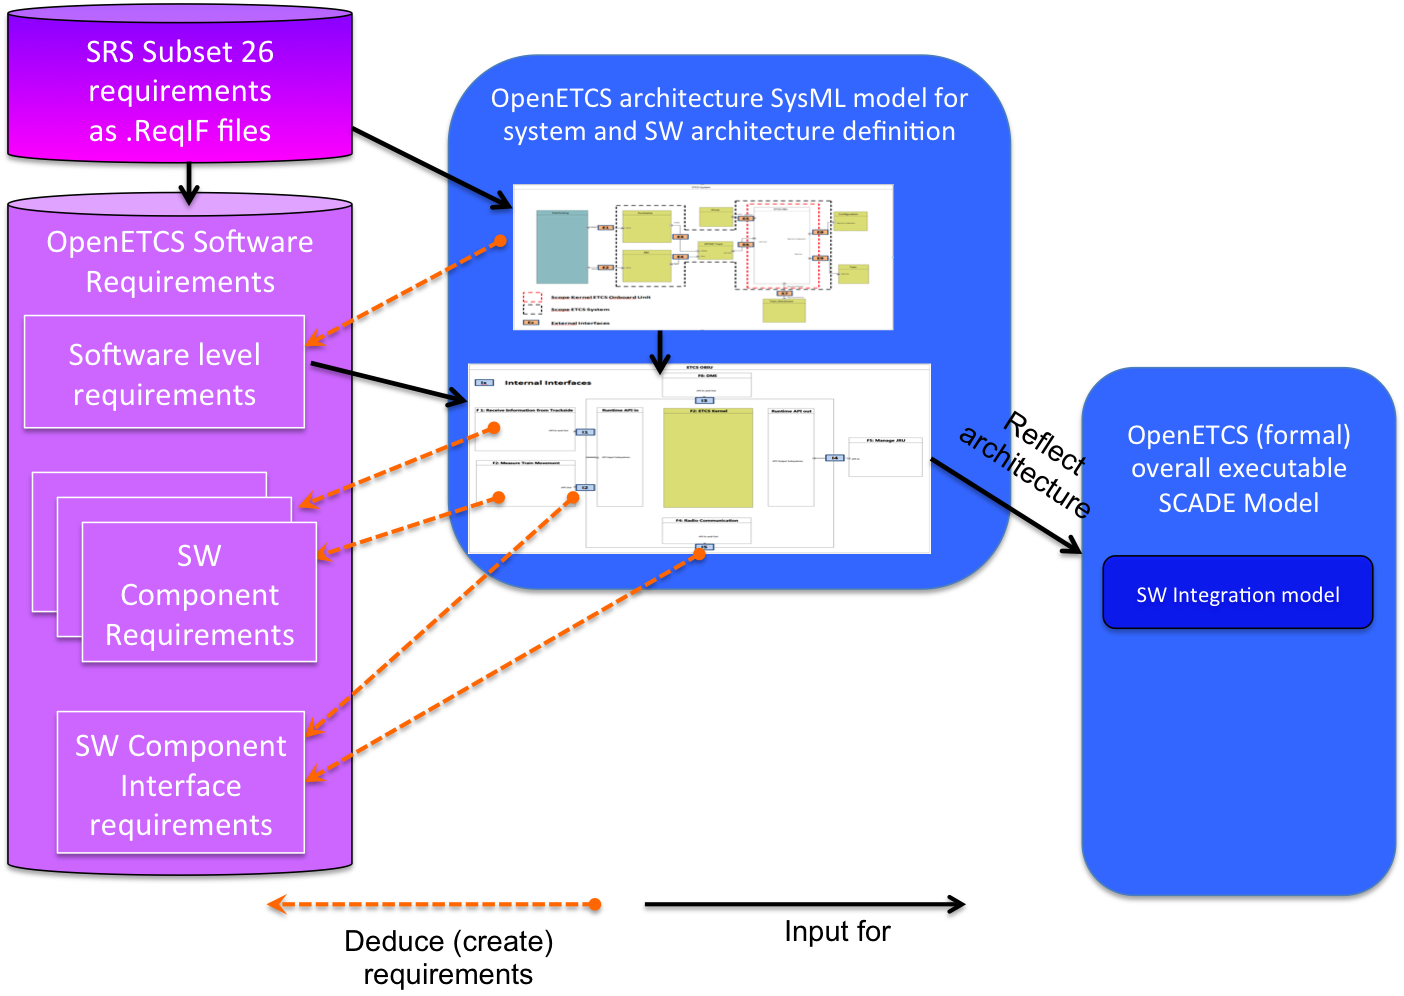
\includegraphics[width=.9\linewidth]
{./images/P2RequirementDerivationWithSysMLModel.png}
\caption{\label{fig:P2RequirementDerivationWithSysMLModel}Software requirements initial definition from SysML model}
\end{figure}



\subsection{P3 - Software Behavior Modeling and Integration Phase}

The phase P3 \textit{Software Behavior Modeling and Integration Phase} cover activities from the EN~50128 development life cycle Software Arch. \& Design Phase (7.3), Software Component Design Phase (7.4) and Software Component Implementation Phase (7.5). 
The overall SCADE model initiated during P2 is refined and enhanced to completely represent Design and Interface Specifications as well as all Component Design Specifications. Source Code in C is generated automatically via the certified SCADE Code Generator and combined with required wrapper software. For these wrapper parts specific development methods have to be defined as these parts are specified.

As this overall SCADE model is composed of several components described by lower level SCADE models and their interfaces, it specifies integration to be performed it can be used as input for SW integration (see P5). This is a "meet in the middle" approach taking as inputs SysML architecture model (top down approach) and functional SW component detailed models (bottom up approach).

\textbf{Note}: \textbf{this Scade overall SW integration model does not appear on current Software development process figure \ref{fig:OpenETCSDevelopmentProcess} in Architecture an Design box and should be present there because it is an important artifact used both as integration of behavioral models (rising part of V cycle applied on models) and as input to prepare integration of software}. Said it differently, there is a small "V" starting with P2 in Architecture and design, descending with P3 in Component Design and rising again in Architecture and Design with P3, still in the descending part of the global V life cycle.

SCADE integration model describes structural but also dynamic integration of component models. It includes at least following elements to consider: 
\begin{itemize}
\item conditions of activation and deactivation of functions (described by component models) through use of modes,
\item Scenarios of functions with control flow including sequencing, branching, merge, fork and synchronization,
\item Arrangement of time events (scheduling), management of asynchronous events
\item Error/exception management to ensure reliability
\item Technical conversion functions to manage exchange of data available in different types/formats
\item Conformance with SysML architecture model?
\end{itemize}

All those SCADE models (low level behavioral models and integration models) provide good input for creation of additional SW component and SW component interface requirements from SCADE operators, blocks, automatons and data types.

The software architecture and design document produced from those SCADE models is also another good input for creation of requirements.

\textbf{But currently neither SCADE models nor Architecture and Design document lead to the creation of requirements in the reference requirements database.} 

Figure \ref{fig:P3RequirementDerivationWithSCADEModels} illustrates what could be done in the future to get a clear SW definition.

\begin{figure}[htbp]
\centering
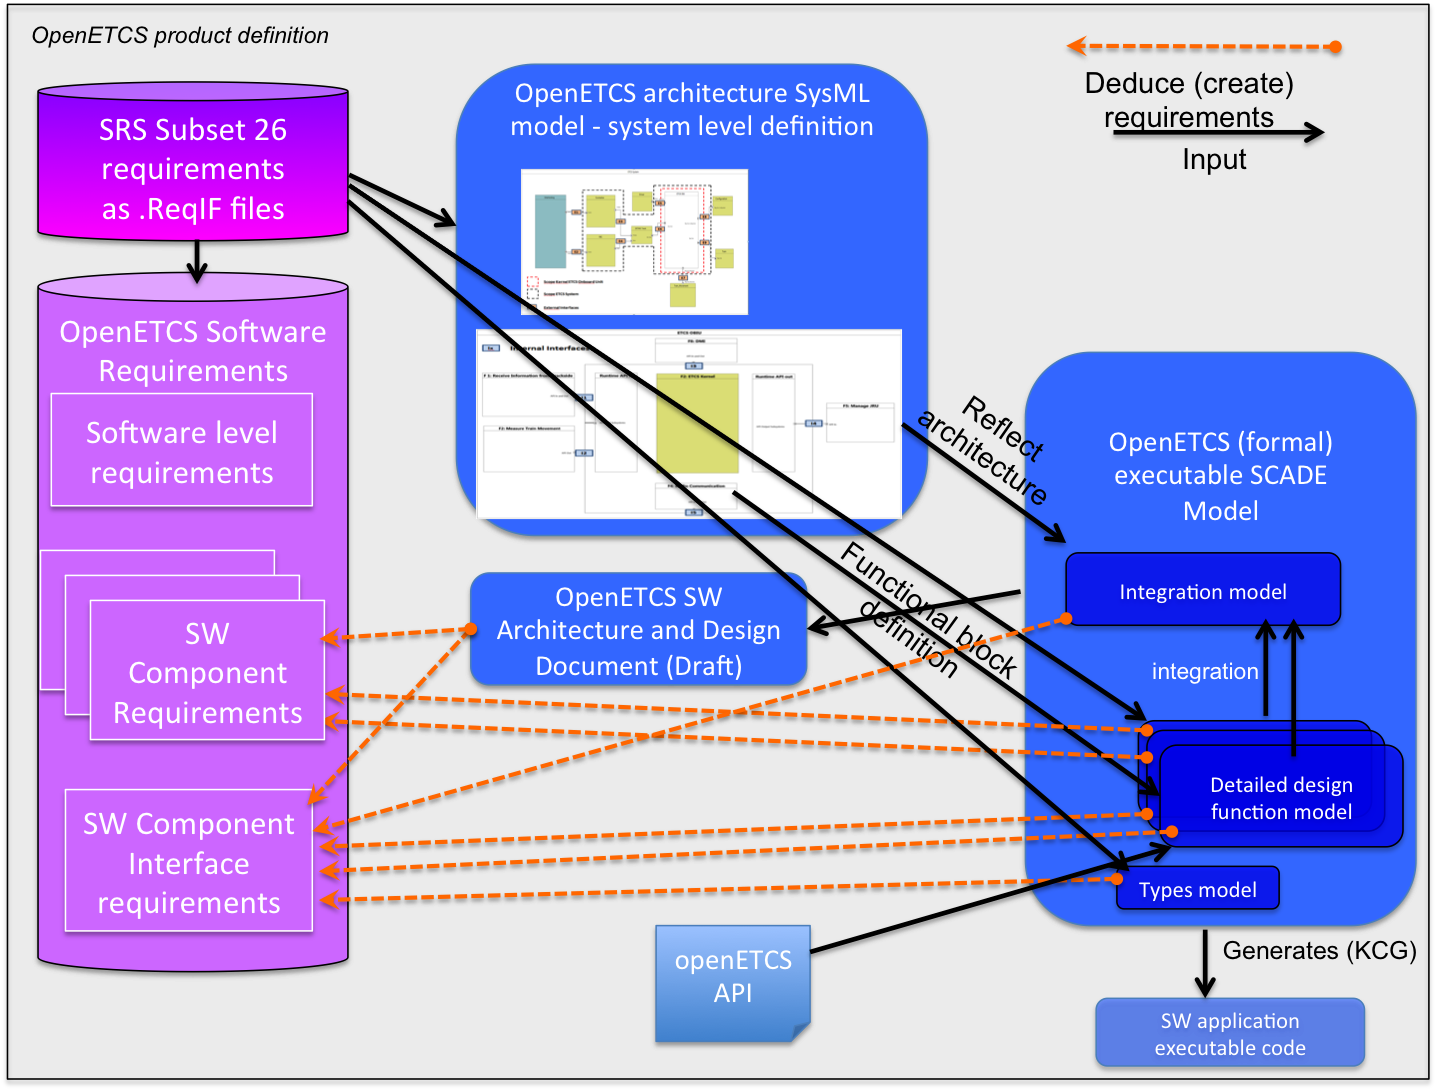
\includegraphics[width=.9\linewidth]
{./images/P3RequirementDerivationWithSCADEModels.png}
\caption{\label{fig:P3RequirementDerivationWithSCADEModels}Software requirements identification from SCADE models and from Software Architecture and design document}
\end{figure}

\subsection{P5 - Formal Validation Phase}

The phase P5 has to cover activities of the Software Component Testing Phase (7.5), Integration Phase (7.6) and mainly Software Validation Phase (7.7) by using simulation, testing and model checking methods. To do so the SCADE environment as well as additional tools are use depending on the specific model property to be tested or proven. 

The Inputs for these activities are the SysML and SCADE models and the C Code.

Currently there is no precise list of traceability links to define and maintain in the frame of this phase.




\chapter{Tool chain current physical architecture solution to support traceability}
\label{sec-5}
\section{Overview of current traceability architecture solution}
This current solution consists in handling requirement management and traceability links through different tools and technologies. The strategy of this approach consists in maximizing efficiency of the different concurrent activities through using tooling locally integrated in the different environments used in the project over its development life cycle (the 5 phases).

As a summary view (will be detailed later) we find:
- P1: ProR is used to support requirement management around a .ReqIf files database
- P2: Scade System is used to edit SysML architecture model from system environment down to software definition and its external interfaces. This model can be displayed in Papayrus SysML and then used by PolarSys ReqCycle tool to create links with .reqIF requirements.
- P3: . ReqIF reference requirements are imported in SCADE and can be traced through the ANSYS RM Gateway based on Reqtify solution. 
- P4: SCADE KCG is used to support generation of C source from SCADE models.
- P5: other tools (to be completed)

Figure \ref{fig:CurrentArchitectureTraceSolution} illustrates current traceability architecture with associated set of tools, scripts and procedures.


\begin{figure}[htbp]
\centering
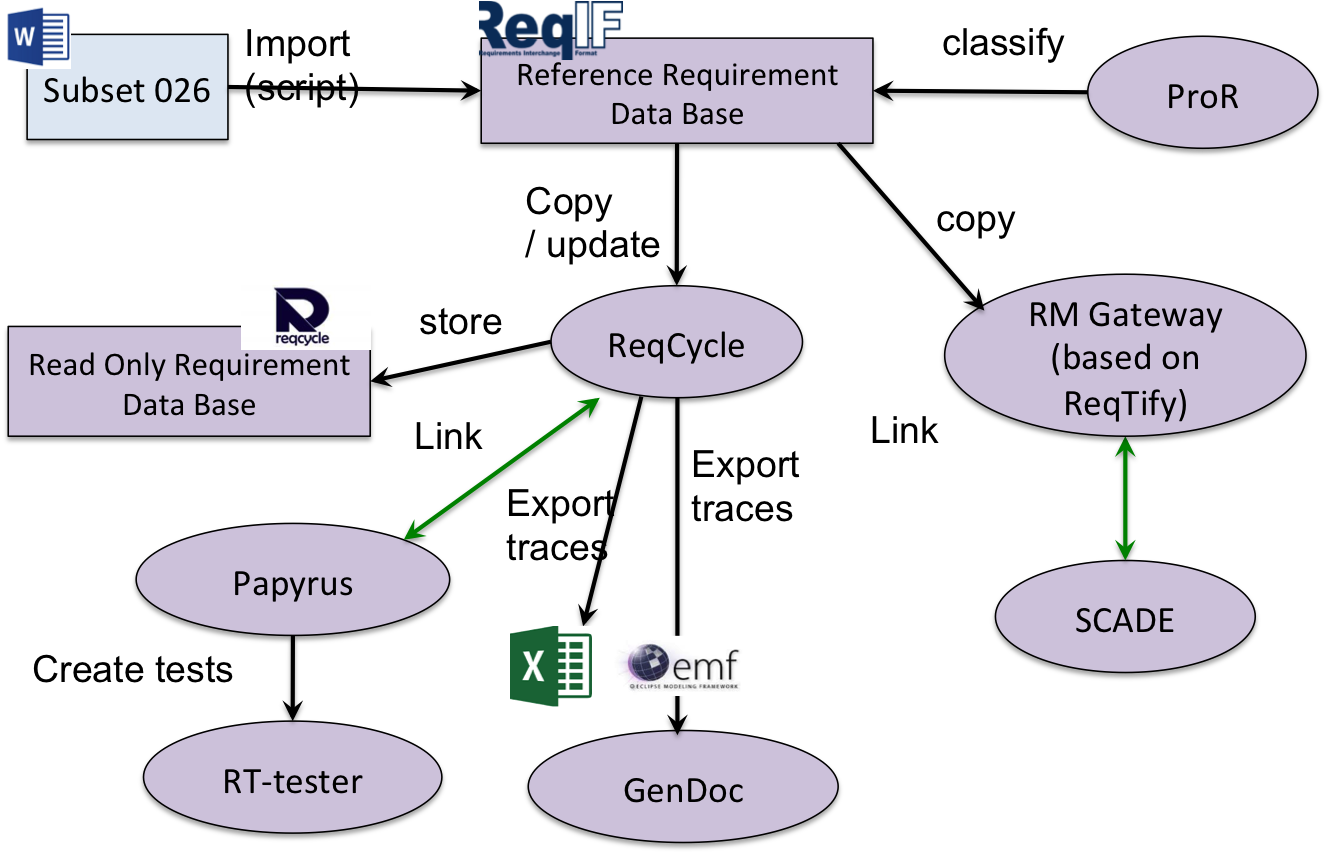
\includegraphics[width=.9\linewidth]{images/CurrentArchitectureTraceSolution.png}
\caption{\label{fig:CurrentArchitectureTraceSolution}Traceability architecture first solution}
\end{figure}

\textbf{Note}: when requirement management tools complete imported requirements, they should guarantee the following rules:
\begin{enumerate}
\item The requirement's structure (hierarchy, scope) is not modified.
\item No requirement should be deleted.
\item Newly added requirements should be either a refinement, derivation or a decomposition of an existing one.
\item The identifier pattern should be respected.
\item Identifiers should remain unique.
\end{enumerate}


\section{P1 phase: ProR, Scade System, Papyrus and ReqCycle}
\subsection{Import of reference requirements through a Script}

Reference Subset 26 input document is converted to a set of ReqIF format files and informally analyses. The analysis specifies relationships between requirements and revised parts of the requirements to obtain a detailed and atomic abstraction level matching the different requirement engineering levels required by Cenelec standards. 

A script is in charge of converting input SRS subset 26 document to requirements in .ReqIF format files. Each requirement has an unique identifier. These identifiers are fixed and cannot be modified by any other
tools.
See \label{importScript} for detailed description of this script, challenges to solve and solutions.

\subsection{Classification of reference requirements through ProR}

ProR is the tool in charge of supporting the requirement classification from this initial set of SUBSET 26 requirements:
\begin{itemize} 
\item filter of requirements to take into account for openETCS project baseline (not all SUBSET 26 requirements are part of openETCS baseline)
\item tag requirements that are considered as software requirements (normally there should be a derivation process that would create SW requirements but it is not the case currently and SW design takes as inputs SUBSET 26 requirements)
\end{itemize}

Currently there is no classification of reference requirements and .reqIf files are an exact translation of the document.

\subsection{Creation of additional requirements through ProR}
ProR is also in charge of supporting creation of additional requirements coming from:
\begin{itemize} 
\item hazard and risks analysis (safety requirements) but we saw that the safety process has been validated through a proof of concept but not yet deployed for the whole project.
\item decomposition (improvement of requirement quality) but this is not done directly in .reqIF files. There is a process called RFC (Request For Comment) in charge of collecting deviations to the SRS subset 26 detected during design. 
\end{itemize}

So finally  .reqIF files only contain SRS subset 26 requirements and no additional requirements are created for now.

\subsection{Link requirements and overall test specification with ReqCycle}
As mentioned in previous chapter, overall test specification is not yet defined but should be linked to the SW requirements and each SW requirement shall precise its verification means (including test specification) and be linked to verification specification (test specification if it is the prefered verification means).

It first means that all requirements shall have an attribute "verificationMeans" taking as possible values "test", "inspection", "analysis" and "demonstration" according to verification plan. We suggest using ProR tool to add this attribute.

It also means that each ReqIF requirement shall have links with at least one of the planned verification means. Tool chain shall support creation of those links and export as a traceability matrix. There are mainly two options with open source solutions:
\begin{itemize} 
\item either use ProR to manage the links with verification specification (mainly test specification) and export associated traceability matrix.
\item else use PolarSys ReqCycle tool to manage those links and export traceability matrix.
\end{itemize}

\label{ReqCycle} 
\textbf{A few words about PolarSys ReqCycle:} this tool was not mature at the beginning of the openETCS projet and was not really available as official open source component from Eclipse. Now this is an official solution from PolarSys industrial Working group from Eclipse foundation and it has followed official Eclipse development and release processes that ensure minimum of quality and transparency in addition to IP analysis. Official description is available here: https://www.polarsys.org/projects/polarsys.reqcycle

In addition, 0.8.0 release has been largely tested and is considered as stable. 
There is Wiki documentation (with development process, user and some tool requirements, installation and tutorial) available here: https://polarsys.org/wiki/ReqCycle

ReqCycle can export traceability links to .csv file and to EMF format model, that can then be used as input by Eclipse gendoc tool to produce an industrial quality level documentation.


\label{toolChoiceForRequirementVerificationLinks}
\textbf{Prefered solution} 
ProR is the simplest approach to get .ReqIF requirements and it can create links, but this approach requires some additional plugin to analyse test definitions from verification specification document.

ReqCycle has to import .ReqIF requirements first before creating traceability links but it is not an issue because there is a ReqIF import connector. Concerning tests, it has a generic document connector able to analyse and extract test definitions if they can be identified through regular expressions, document styles or combine both technics. This connector can also use OCL language and associated queries to identify tests from spreadsheets.

Finally we suggest using PolarSys ReqCycle to support management of links between requirement and test specification because it has all native features/capabilities to import requirements, import test definitions,  create links and export them in a .csv matrix.


\subsection{Update of SRS subset26}
P1 is also concerned by potential changes in reference requirements coming from a new version of SRS subset 26. Any new version should be analyzed for potential impacts on OBU Software. So the tool chain shall be ready to support such update.

Practically it means that it should be possible to compare two versions of .reqIF files created by same import script applied on two different SUBSET 26 versions. That comparison shall lead to a list of deleted requirements, modified requirements (changed text) and new requirements.

From this analysis, the tool chain shall help providing the list of all OBU SW requirements concerned by deleted or updated requirements in order to check associated design and verification specifications (including tests). It means reviewing all traceability links associated to modified .reqIF requirements.

ProR can compare two .reqIF files and then identify changed and deleted requirements. But in order to analyse impact on design and overall test specification, ProR shall access to all those traceability links associated to reference requirements, what is not the case currently.

Can ReqCycle help for that? 
ReqCycle can manage updates of its different requirement sources and list impacts on traceability links. So it might work but under the condition that all tracebility links are captured (created or analysed) by ReqCycle. That is not the case currently.

\textbf{So this point remains open.}
 

\subsection{technical challenges}

\subsubsection{Script description}
\label{importScript}
The \textit{Subset26Import} script generates a hierarchical tree of all traceworthy
artifacts in each chapter of subset-026. Each artifact shall be uniquely addressable via a tracestring.


\label{unique ID definition}
Take the following example:
\begin{figure}[htb]
\centering
\includegraphics[width=.9\linewidth]{images/tracestring-ex.png}
\caption{\label{fig:reqID_ex}Traceability architecture between artifacts}
\end{figure}


\paragraph{Guideline}
The scope of a single requirement ID is a paragraph of text (there are six such
paragraphs in the above example).  requirement IDs are hierarchical. The
hierarchy is a direct mapping of the hierarchy in the original subset-026
text. Levels are separated by a dot. There is a requirement at each level
(i.e. you may truncate the requirement ID to any level and it stays valid).

\paragraph{How to}

Suppose we want to trace the fifth paragraph in the above example i.e
\begin{verbatim}
• End of mission is performed
\end{verbatim}
\begin{enumerate}
\item Let \textsl{traceString} be the variable to store the result.
\item Find the current running number of the base list. That is the list which
includes the chapter number. In this example this number equals
\verb+3.5.3.7.+ Set \textsl{traceString} to this number.
\item Count the number of paragraphs in this list item starting with 1 and append
this number in square brackets to the \textsl{traceString} if it is greater than 1.

Note: For the first iteration in the example there is only one such paragraph
(\texttt{If the establishment...}). Hence, we do not append anything. In the
second iteration there are two such paragraphs (\texttt{The on-board shall...} and
\texttt{If this request is not ...}). Hence, the second one will receive an
\texttt{[2]} appendix.

\item Until you arrived at your target paragraph: Append any running number of
sub-lists and remove leading or trailing characters (such as braces). If the
current sub-list is bulleted then the level string always becomes
\verb+[*][n]+ (with n being the running number of that bullet starting at
1). Prefix this new level with a dot (\verb+.+) and append it to the
\textsl{traceString}.

Note: \verb+a)+ is the identifier of one such sub-list item. The trailing brace
will be removed. The bullet points form another (less significant) sub-list.
\item Do step 3.
\item Do step 4 or break.
\item \textsl{traceString} is now the fully qualified requirementID.
\end{enumerate}

This will result in the following requirement ID: \quad \verb+3.5.3.7.a[2].[*][2]+



\section{P2 phase: ProR, Scade System, Papyrus and ReqCycle}

Concerning P2, main traceability links concern verification of SW architecture. 

\subsection{verification of SW architecture through ReqCycle}

Architecture model is defined with a subset of SysML language (blocks definition and internals) through Scade System tool.
We want to trace this architecture to the reference requirements that are imported (translated) subset 26 requirements.

3 options could be considered to support creation of this traceability:
\begin{enumerate} 
\item \textbf{traceability in Scade System environment through the Ansys RM Gateway based on Dassault Systems Reqtify product}: .ReqIF requirements are imported in the RM Gateway (through Reqtify configuration) and Scade System provides a way to reference those requirements from blocks or connectors that define architecture. The RM Gateway creates the links and exports a traceability matrix.
\item \textbf{traceability in ProR through dedicated ProR-Papyrus proxy module}: SysML model created with Scade System can be displayed with Papyrus open source tool. ProR is used to create traceability links to model elements from Papyrus thanks to a special configuration and a proxy module (see https://github.com/openETCS/toolchain/wiki/User-Documentation) .
\item \textbf{traceability through PolarSys (Eclipse-based) ReqCycle tool}: we use same previous approach to see SysML model initiated by Scade System in Papyrus tool. Then .ReqIF files are imported through a ReqCycle import connector and made available as ReqCycle requirements (in pivotal eclipse modeling format). Traceability links are created by traceability creator or Drag and drop features available in ReqCycle to link reqCycle requirements and any EMF model including Papyrus SysML. Requirements and traceability progress can be visualized in ReqCycle and traceability data can be exported to .csv file.
\end{enumerate}

Option 1 relies on closed source technology (RM Gateway) and there are licensing issues.
Option 2 relies on specific proxy ProR module developed during the project: require adapters from both ProR and Papyrus and maintenance is not guaranteed over time (not core part of both roadmaps).
Option 3 relies on native features from ReqCycle tool:  a ReqIF connector to import .ReqIF requirements and native commands like traceabilityCreator view to trace requirements with EMF models including Papyrus (see \ref{ReqCycle traceability}) 

Option 3 is considered today as best option to support traceability concerning SW architecture verification.


Architecture is initialized by SysML model and then reflected and completed in SCADE model. So question becomes: what is input for traceability with requirements? SysML model or SCADE model?

 So we suggest creating links from SysML architecture model. With that approach we can use ReqCycle (tool has been briefly presented previously - see  \ref{ReqCycle}).


\subsection{Creation of traceability links between a requirement and a Papyrus SysML with ReqCycle}
\label{ReqCycle traceability}

Figure \ref{fig:ReqCycleTraceabilityCreator} illustrates a simple way to create a link between a reference requirement and a model element through ReqCycle traceability creator view.


\begin{figure}[htbp]
\centering
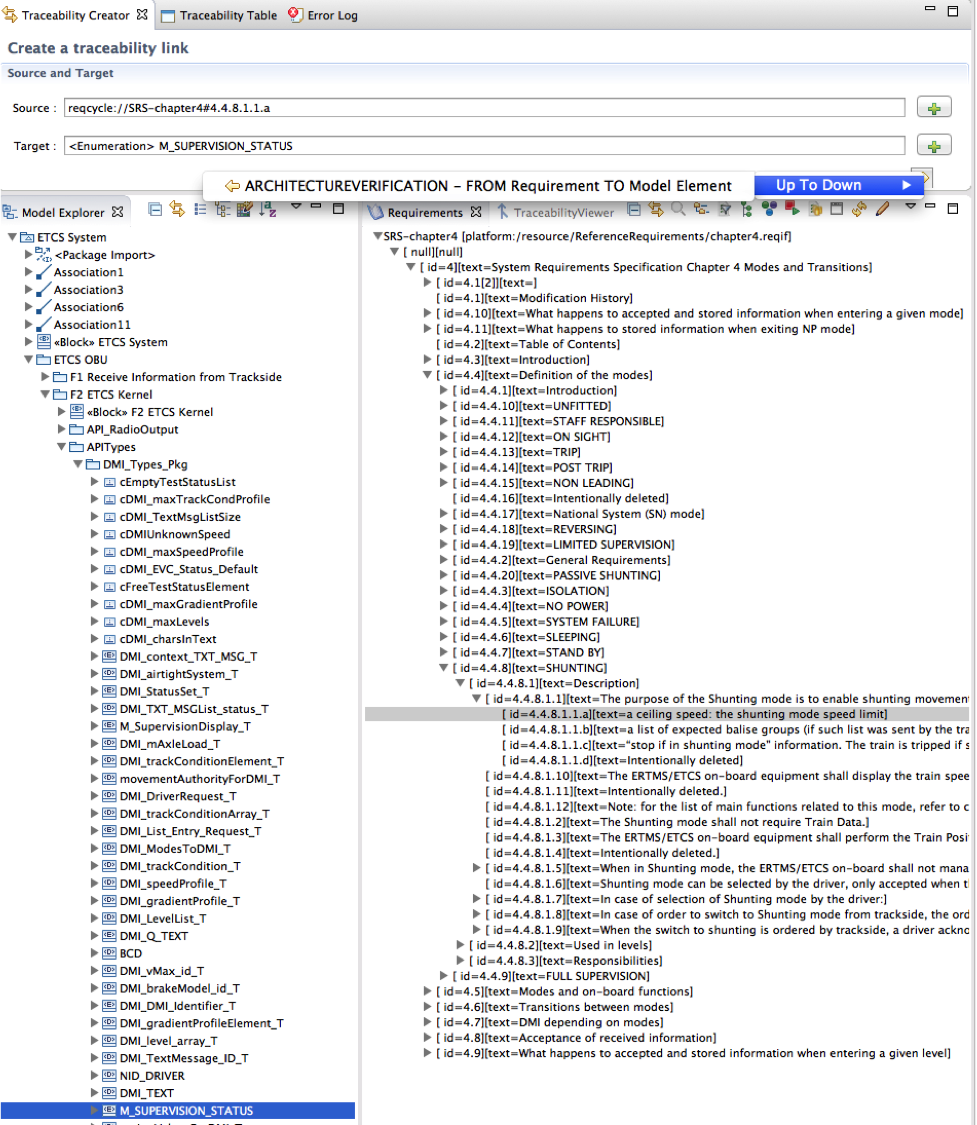
\includegraphics[width=.9\linewidth]{images/ReqCycleTraceabilityCreator.png}
\caption{\label{fig:ReqCycleTraceabilityCreator}Creation of links with Reqcycle between requirements and Papyrus}
\end{figure}


\section{P3 phase: ProR, Scade suite and ???}
SysML brings top level decomposition architecture staring from openETCS system while SCADE model brings bottom up SW architecture coming from integration of behavioral SCADE models.
So when we look at SW detailed architecture and at behavioral models, the reference is SCADE, not SysML. So we need to be able to trace all detailed design elements from SCADE behavioral models and all other design elements associated to their integration at upper level. All those elements have to be traced to the reference requirements. 

From SCADE the only serious option today is to use the proprietary ANSYS RM Gateway but there is licensing issue for some partners. So currently this is not ideal solution and there is no real support of traceability for SCADE model elements today.

One option exists but it has not been investigated seriously for now: using SCADE Eclipse API to export SCADE models to Eclipse EMF Format and then use ReqCycle to perform traceability as ReqCycle has native commands to create links between any requirement and EMF model elements. We do not consider this option in this document and rather select it as an improvement axis.

\section{P4 phase: SCADE suite and Scade KCG}
Traceability between SCADE model and C source code is ensured by SCADE KCG.

\section{P5 phase: Verification and validation of SW product}
Currently no traceability relations have been clearly defined.

\chapter{Limits of current traceability architecture and axes of investigation for improvement}
\label{sec-6}

\section{Current identified limits}
Before looking at possible alternative software solutions to support traceability in the different phases, let us come back to the choices in terms of artifacts to trace.
\subsection{Limits concerning the baseline of requirements used as input for traceability}

Currently only SRS subset requirements are considered in the creation of traceability links. But there are also other sources of requirements including openETCS API, CENELEC standards and user stories. How to ensure traceability to those artifacts if they are not integrated into the reference requirements database?

Secondly, with \textit{traditional} SRS requirements derivation down to SW requirements, the method consists in decomposing functional requirements and then allocating them to lower level design elements and so on down to Software level. 
At Software level, then we trace software architecture elements to software requirements through a "satisfy" semantics trace.
Finally we have different steps in the creation of  traceability links and all created links have "simple" semantics ("satisfy" or "allocation") that can be validated quite easily.

in P1, we trace directly architecture elements (SysML model) to SUBSET 26 requirements instead of tracing them to openETCS SW requirements derived from System requirements also derived from SUBSET 26 requirements. The consequence is that the trace links are harder to validate because they sometimes connect elements of very different engineering levels.

Finally we strongly recommend three things:
- think about other scripts or solutions to import other reference stakeholder requirements including at least openETCS API and user stories (CENELEC standards can be traced manually) to improve traceability to its reference sources.
- add a tag to all reference requirements with identification of a level to clearly identify SW requirements and those that are from a higher level.
- provide a rationale to the trace link, at least concerning all requirements that are not clearly identified as software requirements, to give understanding elements to the future reviewers (next review or perhaps in several months when Subset 26 version will change).

\subsection{Limits concerning additional requirements}
We already mentioned the SRS requirements derivation process not done but there are also other requirements that should be created during SRS analysis: safety requirements, as a result from risk and hazard analysis.

When considering that openETCS are only requirements coming as inputs, we can take the assumption that we never change them and consider all requirements as "read only" requirements. We do not look into the issues of managing (import, export, synchronization...) additional requirements potentially created by other tools like EventB or another tool.

\subsection{Limits concerning traceability with SysML elements}
For verification of SW architecture we have considered that SysML model was representative and that we could then create traceability links with sysML model elements. What happens if overall SCADE model is not aligned with SysML model concerning architecture? then traceability links with SysML model will be false and review cannot see that.

So, in order to continue trusting links done with SysML model we must ensure that architecture designed with SysML is reflected in overall SCADE Model and that any modification on architecture done at SCADE side is reflected back to the SysML model. Said it differently there must be architecture synchronization between both models. If there is no way to check that synchronization, some links done to verify architecture might be wrong without ability to notice that.


\subsection{Limits concerning traceability with SCADE elements}
Currently there is no satisfying solution to trace SCADE model elements to reference .ReqIF elements. Some use the RM gateway but others do not for licensing reason and finally it puts some risk on the project not to be able to verify software detailed design.


\subsection{Limits concerning management of all traceability links}
We saw in previous chapter that in case of update of SRS Subset 26 ProR will be able to provide a diff between requirements but will probably not be able to list all associated traceability links that have to be checked and handled (removed or confirmed or completed).
That is another issue to investigate.

\section{Investigation axes for improvements}
We suggest different investigation axes to manage main limits identified previously. 
Those investigations will be detailed and will lead to results reported into an other document.

\subsection{Ability to export Scade model as Eclipse EMF model}
Esterel Technologies explains in their SCADE documentation that it is possible to export SCADE into Eclipse Modeling Framework format through their Eclipse API: see http://www.esterel-technologies.com/products/scade-suite/software-prototyping-desgin/scade-suite-advanced-modeler/

With that approach it would become possible to see SCADE exported models in the Eclipse environment and create links through ReqCycle traceability engine (ReqCycle can trace requirements to EMF models without needing a new adapter).

This is the most urgent investigation axis to look at. If it provides good results, then ReqCycle can be used to manage most important links in openETCS project and can be considered as reference tooling for traceability with ability to aggregate all links. It simplifies architecture and answers to the last two limits identified previously.
 
\subsection{Combined solution for requirement management and traceability tools}
Concerning requirement management and traceability there exist mainly two open source Eclipse based solutions: ProR and ReqCycle. 
RMF/ProR is the natural choice for OpenETCS to support requirement management while ReqCycle is a good choice to support management of traceability links (creation, capture, visualization and export).

It would be interesting to investigate on a second architecture solution combining ProR and ReqCycle as reference tooling to manage both requirements and traceability links in an integrated way. 


\begin{figure}[htb]
\centering
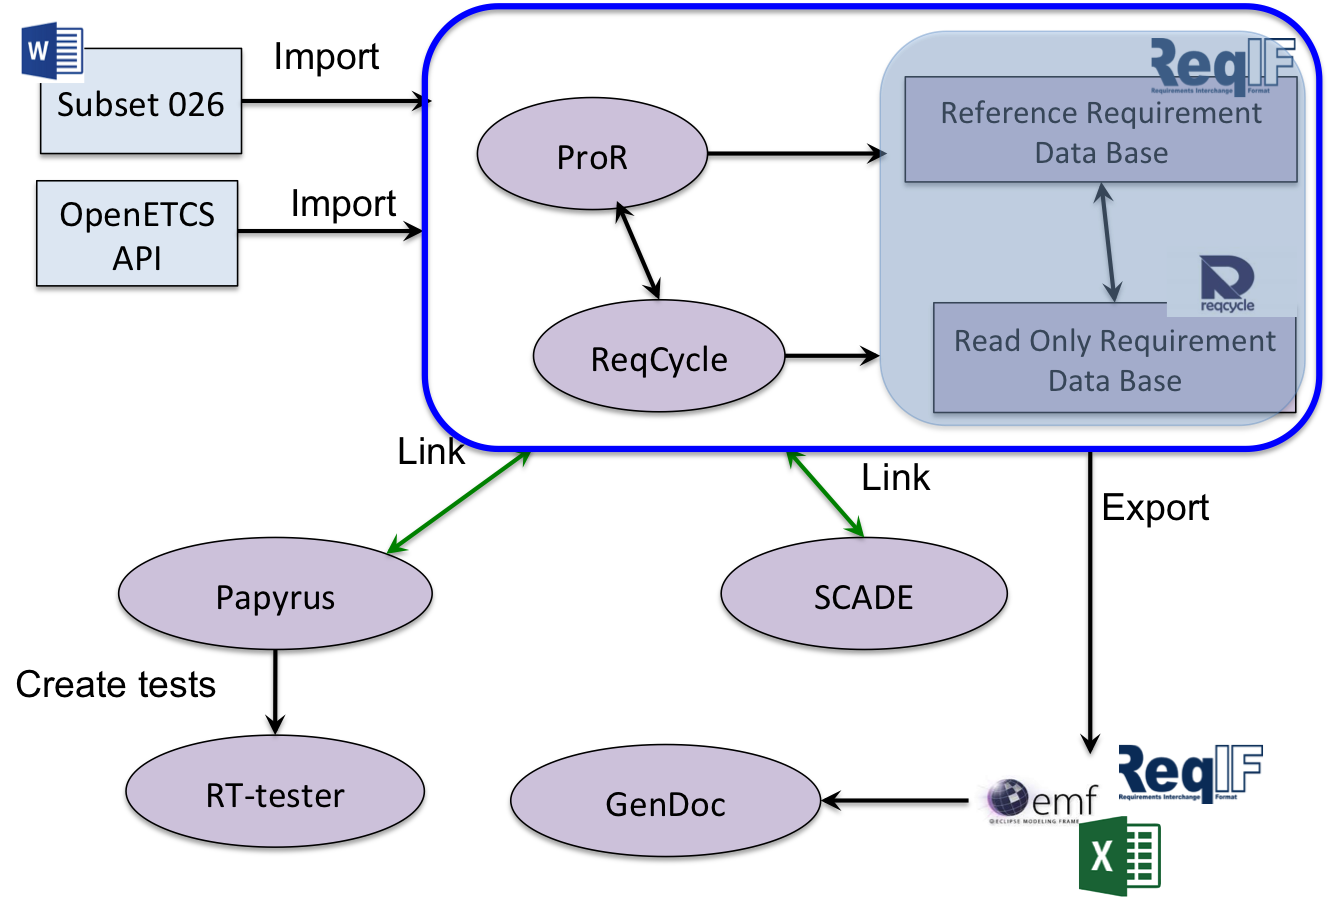
\includegraphics[width=.9\linewidth]{images/second_trace_solution.png}
\caption{\label{fig:trace_second}Traceability architecture second solution}
\end{figure}

With that approach, there is still one master reference requirements data base entirely managed by ProR. Requirement database is initialized by import from the subset-026 word document, as in solution 1 (see \ref{sec-5-1}) and by import from OpenETCS API.
All new OpenETCS requirements are added in this requirement database through ProR tool.

Traceability is managed by ReqCycle tool. In order to ease visual selection of requirements in ReqCycle, there is a copy (could be a link) of reference requirements hierarchy into a ReqCycle database. Then ReqCycle manages links with Papyrus and links with SCADE. 
Finally, traceability can be exported by ReqCycle and processed by Gendoc tool to deliver documentation.


\subsection{ReqCycle used as centralized solution and ProR for requirement edition}
This third solution consists in using only one centralized Requirement database (as in previous solutions) managed by one eclipse-based solution (ReqCycle) also used to support requirement traceability for all models (Papyrus and SCADE). ProR is used to classify and edit requirements instead of ReqCycle basic requirement editor.

\begin{figure}[htb]
\centering
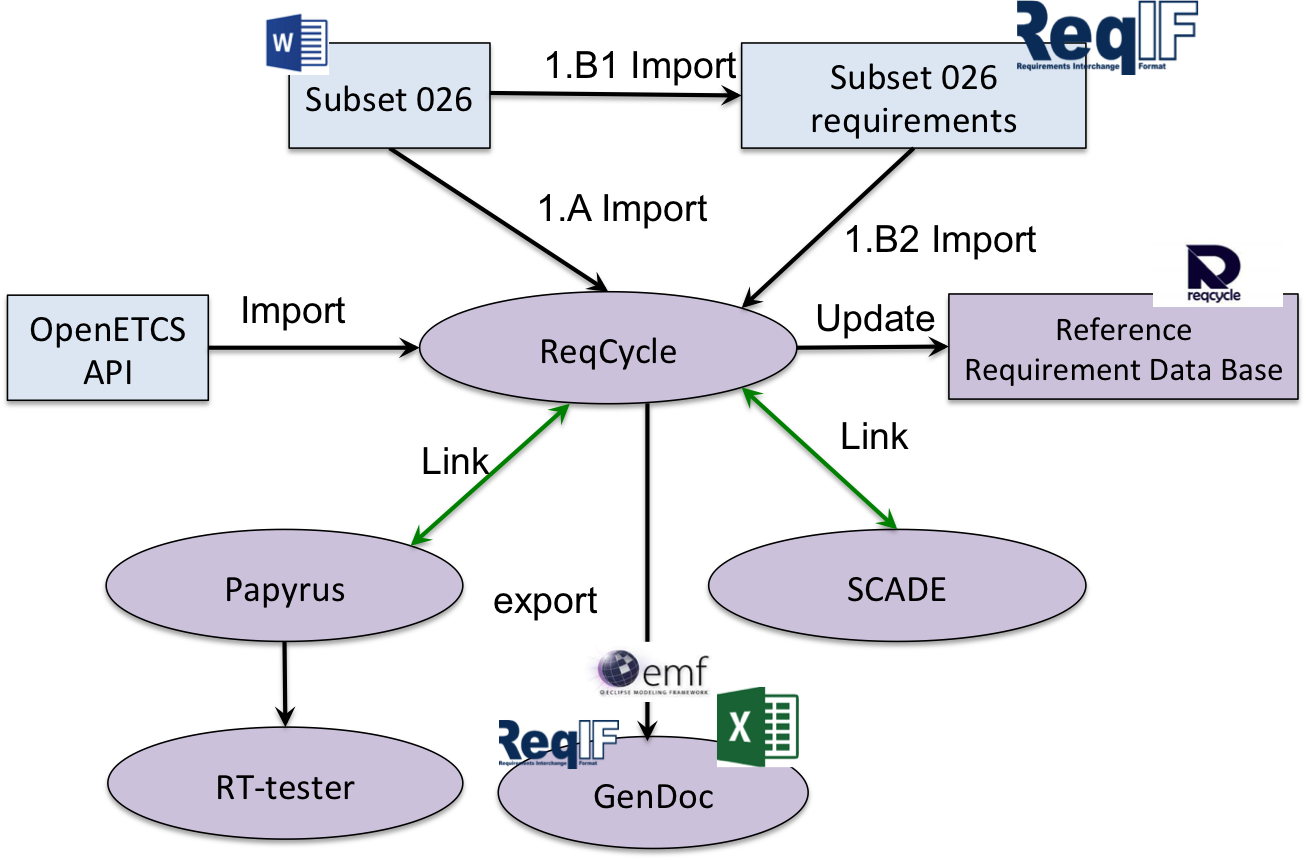
\includegraphics[width=.9\linewidth]{images/Third-Solution-ReqCycle.png}
\caption{\label{fig:trace_third}Traceability architecture third solution with ReqCycle only}
\end{figure}

With that approach, there is still one master reference requirements data base entirely managed by ReqCycle. Requirement database is initialized by import from the subset-026 word document through two possible means (see next section) and by import from OpenETCS API.
All new OpenETCS requirements are added in this requirement database through ReqCycle tool that delegates requirement edition to ProR.






%% Bibliography
% \nocite{*}
\bibliographystyle{unsrt}
\bibliography{oetc_WP7_Traceability}



%Examples are below


%\lipsum[11]

%\nocite{*}

%\bibliographystyle{unsrt}
%\bibliography{Lbrr}



% \begin{thebibliography}{9}

% \bibitem{lamport94}
%   Leslie Lamport,
%   \emph{\LaTeX: A Document Preparation System}.
%   Addison Wesley, Massachusetts,
%   2nd Edition,
%   1994.

% \end{thebibliography}

%===================================================
%Do NOT change anything below this line
\end{document}

%%  LocalWords:  traceability OpenETCS
